\documentclass[a4paper,12pt]{report}

% Carica pacchetti necessari
\usepackage{algorithm}
\usepackage{algpseudocode}
\usepackage{eurosym}
\usepackage{bbm}
\usepackage{multicol}
\usepackage{hyperref} % Per rendere i riferimenti cliccabili
\usepackage{amsmath}   % Per le equazioni e la matematica avanzata
\usepackage{amssymb}   % Per simboli matematici come \mathbb{R}
\usepackage{amsfonts}  % Per font matematici aggiuntivi
\usepackage{graphicx}  % Per includere immagini
\usepackage{fancyhdr}   % Per le intestazioni personalizzate
\usepackage[backend=biber, style=numeric]{biblatex}  % Per la bibliografia
\usepackage[italian]{babel}
\usepackage{caption}
\usepackage{subcaption}
\usepackage{csquotes}
\usepackage{listings}
\usepackage{xcolor}
\usepackage{adjustbox}
\usepackage{url}
\usepackage{textcomp}
\lstset{
    basicstyle=\ttfamily,
    keywordstyle=\color{blue},
    commentstyle=\color{gray},
    stringstyle=\color{red},
    numbers=left,
    numberstyle=\tiny,
    stepnumber=1,
    numbersep=5pt,
    showstringspaces=false,
    breaklines=true,
    frame=single
}
\addbibresource{bibliografia.bib}  % Il nome del file .bib per la bibliografia
\makeatletter
\renewcommand{\ALG@name}{Algoritmo} 
\makeatother
\renewcommand{\theequation}{\arabic{equation}}
\usepackage{chngcntr}
\counterwithout{equation}{chapter}

% Inizio del documento
\begin{document}

% Prima pagina
\begin{titlepage}
\centering

\vspace*{0.5cm}

% Logo

\includegraphics[width=0.20\textwidth]{logo_unisalento.png}

\vspace{0.8cm}

% Università, facoltà, corso
{\Large\textsc{Università del Salento}}\\[0.3cm]
{\large Facoltà di Ingegneria}\\[0.15cm]
{\large Corso di Laurea in Ingegneria dell'Informazione}

\vspace{0.6cm}
\rule{0.8\textwidth}{0.4pt}

\vspace{1.2cm}

% Titolo
{\LARGE\bfseries
ChillChain --- Piattaforma IoT per il\\[0.3cm]
trasporto refrigerato condiviso
}

\vspace{0.6cm}

{\large\itshape Matching domanda-offerta e rilevazione anomalie\\[0.15cm]
con LSTM Autoencoder}

\vspace{1.5cm}

% Relatore e candidato
\begin{minipage}[t]{0.45\textwidth}
\raggedright
{\small\textsc{Relatore}}\\[0.2cm]
{\normalsize Prof. Luigi Patrono}\\[0.5cm]
{\small\textsc{Tutor}}\\[0.2cm]
{\normalsize Ing. Teodoro Montanaro}
\end{minipage}%
\hfill
\begin{minipage}[t]{0.45\textwidth}
\raggedleft
{\small\textsc{Studente}}\\[0.2cm]
{\normalsize Antonio Bello}\\[0.15cm]
{\small Mat. 20093232}
\end{minipage}

\vfill

\rule{0.8\textwidth}{0.4pt}\\[0.4cm]
{\normalsize Anno Accademico 2025--2026}

\end{titlepage}

% Indice (automatico)
\tableofcontents
\newpage

\chapter{Introduzione}
\label{ch:introduzione}

La gestione della catena del freddo rappresenta una delle sfide più critiche nel settore della logistica. Il trasporto di merci deperibili richiede il mantenimento rigoroso di condizioni ambientali controllate lungo l'intera filiera distributiva, dalla produzione alla consegna finale. Anche una breve deviazione dalla temperatura richiesta può compromettere irrimediabilmente la qualità e la sicurezza dei prodotti trasportati, con conseguenze economiche rilevanti e potenziali rischi per la salute pubblica. 

A rendere il problema ancora più complesso contribuisce la frammentazione del mercato del trasporto refrigerato: da un lato, le aziende di trasporto gestiscono flotte di veicoli che spesso viaggiano con capacità parzialmente inutilizzata; dall'altro, i clienti che necessitano di spedire piccoli quantitativi si trovano costretti o a sostenere costi elevati per soluzioni FTL (\textit{Full Truckload} ovvero il noleggio di un intero veicolo refrigerato) o a ricorrere a soluzioni LTL (\textit{Less Than Truckload}, ovvero spedizioni che condividono il veicolo di trasporto con altri carichi e che vengono consolidate in centri di smistamento intermedi), che comportano molteplici passaggi in magazzino, tempi di consegna più lunghi e un rischio maggiore di rottura della catena del freddo. 

Le soluzioni attualmente disponibili sul mercato affrontano questi problemi in modo parziale e disgiunto. Piattaforme come Flock Freight \cite{flockfreight2024} hanno introdotto il concetto di \textit{Shared Truckload} (STL), sfruttando algoritmi di intelligenza artificiale per consolidare spedizioni di clienti diversi su uno stesso veicolo e ottimizzare le rotte in maniera automatica. A differenza delle spedizioni LTL tradizionali, il carico viaggia sullo stesso veicolo lungo l’intero percorso, evitando passaggi intermedi nei centri di smistamento. 

Sul versante del monitoraggio, le soluzioni IoT per la \textit{cold chain} come Lynx Fleet \cite{carrierlynx2024} operano tipicamente come sistemi B2B, scollegati dalla fase commerciale di prenotazione e pricing, e si limitano per lo più a un monitoraggio basato su soglie statiche che, pur essendo semplice da implementare, non è in grado di rilevare pattern anomali complessi dell'impianto di refrigerazione.

Il presente lavoro propone \textbf{ChillChain}, una piattaforma IoT che integra in un'unica soluzione il matching tra domanda e offerta di spedizioni refrigerate e il monitoraggio intelligente della catena del freddo con rilevazione automatica delle anomalie. L'idea alla base del progetto è consentire ai clienti di visualizzare i viaggi già programmati compatibili con le proprie esigenze di spedizione e scegliere a quale viaggio aggregare la propria spedizione. La rotta del veicolo viene ricalcolata dinamicamente per includere le nuove fermate, mentre un sistema di pricing basato sull'occupazione del mezzo applica un divisore esponenziale che rende il costo per singolo cliente progressivamente più conveniente all'aumentare delle spedizioni condivise, incentivando così un utilizzo più efficiente della capacità di trasporto.

Accanto alla componente di marketplace, la piattaforma integra un sistema di monitoraggio in tempo reale dei parametri operativi dei veicoli refrigerati. I dati telemetrici vengono trasmessi via MQTT e analizzati da un servizio dedicato di rilevazione anomalie. Quest'ultimo impiega un LSTM Autoencoder, addestrato sul comportamento nominale dell'impianto, per calcolare l'errore di ricostruzione di ciascuna finestra temporale di osservazione: quando tale errore supera una soglia appresa in fase di training, il sistema genera una notifica che viene inoltrata al tecnico responsabile attraverso la dashboard della piattaforma.

Dal punto di vista architetturale, ChillChain adotta un'architettura a microservizi composta da un backend Spring Boot che gestisce la logica applicativa e le API REST, un frontend React per l'interfaccia utente, un broker MQTT Mosquitto per la comunicazione in tempo reale, due servizi Python dedicati rispettivamente allo streaming dei dati telemetrici e alla rilevazione delle anomalie, e un database MongoDB per la persistenza. L'intera infrastruttura è orchestrata tramite Docker Compose, garantendo riproducibilità e semplicità di deployment. L'obiettivo del progetto è dimostrare la fattibilità di un approccio integrato che unisca la dimensione commerciale della logistica collaborativa con quella tecnica del monitoraggio.
\chapter{Analisi dei Requisiti}
\label{ch:requisiti}

In questo capitolo vengono descritti i requisiti funzionali e non funzionali che il sistema ChillChain è chiamato a soddisfare. L'analisi è stata condotta considerando i tre profili utente previsti dalla piattaforma --- amministratore, cliente e tecnico.

\section{Requisiti Funzionali}

I requisiti funzionali definiscono le capacità operative che la piattaforma deve offrire ai propri utenti e descrivono il comportamento atteso del sistema in risposta a specifiche azioni o eventi.

\subsection{Gestione degli utenti e autenticazione}

Il sistema deve consentire l'autenticazione mediante credenziali protette. A ogni utente autenticato viene assegnato un ruolo tra amministratore e tecnico. Il cliente non ha bisogno di autenticazione.

\subsection{Gestione della flotta}

L'amministratore deve poter registrare nuovi veicoli nella piattaforma, specificando per ciascuno le dimensioni del vano di carico (larghezza, altezza, lunghezza), la portata massima in peso, il costo per chilometro e l'indicazione sulla presenza o meno dell'impianto di refrigerazione. Il sistema deve consentire la visualizzazione dell'intera flotta e la rimozione dei veicoli non più operativi.

\subsection{Gestione dei viaggi e delle spedizioni}

L'amministratore deve poter visualizzare l'elenco dei viaggi programmati e consultare le spedizioni associate a ciascun viaggio.

\subsection{Ricerca e prenotazione delle spedizioni}

Il cliente deve poter ricercare i viaggi disponibili inserendo l'indirizzo di partenza, l'indirizzo di arrivo, le caratteristiche del proprio pacco --- dimensioni, peso, necessità di refrigerazione --- e la data entro cui la consegna deve essere completata. 
Il sistema deve restituire due categorie di risultati: nuovi viaggi, generati a partire dai veicoli della flotta ancora privi di viaggi assegnati con percorso calcolato ad hoc, e viaggi condivisi, corrispondenti a viaggi già programmati che dispongano di capacità residua sufficiente e di compatibilità geografica con il percorso richiesto. Per i viaggi condivisi, il prezzo deve essere ricalcolato applicando un meccanismo di divisione basato sul numero di spedizioni già presenti, in modo da incentivare la condivisione del veicolo. Il cliente seleziona il viaggio desiderato tra quelli proposti. Alla conferma della selezione, il sistema deve: nel caso di un nuovo viaggio, crearlo automaticamente con il percorso calcolato; nel caso di un viaggio condiviso, ricalcolare dinamicamente il percorso introducendo le fermate del nuovo cliente come tappe intermedie.

\subsection{Monitoraggio telemetrico in tempo reale}

Il sistema deve acquisire i dati telemetrici provenienti dai sensori installati a bordo dei veicoli refrigerati. Il tecnico deve poter visualizzare i dati telemetrici attraverso una dashboard che presenti l'andamento temporale dei parametri mediante grafici, con la possibilità di filtrare per veicolo e per tipologia di dato telemetrico.

\subsection{Rilevazione delle anomalie}

Un servizio dedicato deve analizzare in maniera continuativa i flussi telemetrici provenienti dai veicoli e identificare automaticamente condizioni anomale. Quando un'anomalia viene confermata, il sistema deve generare una notifica persistente, associata al veicolo interessato.
\subsection{Gestione delle notifiche}

Il tecnico deve poter consultare l'elenco delle notifiche ricevute, ciascuna contenente il nome del veicolo, il timestamp dell'evento, l'errore di ricostruzione e un messaggio descrittivo dell'anomalia rilevata. 
\section{Requisiti Non Funzionali}

I requisiti non funzionali specificano le qualità architetturali e operative che il sistema deve garantire trasversalmente rispetto alle singole funzionalità.

\subsection{Usabilità}

L'interfaccia utente deve essere progettata con particolare attenzione alla chiarezza e all'immediatezza d'uso. Le informazioni devono essere presentate in modo differenziato in base al ruolo dell'utente.

\subsection{Sicurezza}

Il sistema deve proteggere le comunicazioni tra client e server mediante autenticazione e assegnazione dei ruoli agli utenti autenticati. Le password degli utenti devono essere memorizzate in forma cifrata. 

\subsection{Modularità e manutenibilità}

L'architettura del sistema deve seguire il paradigma a microservizi, con una separazione netta tra le componenti applicative. Ogni componente deve poter essere sviluppato, testato e aggiornato indipendentemente dagli altri.

\subsection{Portabilità e riproducibilità del deployment}

L'intera infrastruttura deve essere containerizzata tramite Docker e orchestrata mediante Docker Compose, in modo da garantire che il sistema possa essere avviato in maniera identica su qualsiasi macchina che disponga del runtime Docker.

\chapter{Stato dell'Arte}
\label{ch:stato-arte}

In questo capitolo vengono analizzate le principali soluzioni esistenti nel panorama della logistica collaborativa, del monitoraggio IoT della catena del freddo e della rilevazione di anomalie su serie temporali. Per ciascuna soluzione viene fornita una descrizione sintetica, seguita da un'analisi critica che ne evidenzia i limiti rispetto alla proposta presentata in questo lavoro.

\section{Flock Freight -- FlockDirect\textsuperscript{\textregistered} Shared Truckload}

Flock Freight è un'azienda statunitense che ha introdotto il concetto di \textit{Shared Truckload} (STL), una modalità di spedizione che consente di consolidare carichi di clienti diversi su un unico camion mediante una tecnologia brevettata basata su intelligenza artificiale. L'algoritmo di Flock Freight analizza posizioni geografiche, calendari di spedizione e dimensioni dei carichi per individuare, tra miliardi di combinazioni possibili, gli abbinamenti più efficienti, instradando il veicolo su percorsi diretti e privi di soste in magazzini intermedi \cite{flockfreight2024}. A differenza del tradizionale LTL (\textit{Less Than Truckload}), in cui la merce viene scaricata e ricaricata più volte lungo il percorso, nello STL il carico non lascia mai il veicolo fino alla consegna, riducendo drasticamente il rischio di danneggiamento e i tempi di transito. Flock Freight dichiara consegne puntuali nel 97\% dei casi e un tasso di danneggiamento 5,4 volte inferiore rispetto all'LTL, con una riduzione delle emissioni di CO\textsubscript{2} fino al 40\%.

Nonostante la solidità della soluzione, il modello di Flock Freight presenta caratteristiche differenti rispetto all'approccio proposto in ChillChain. Dal punto di vista dell'ottimizzazione, Flock adotta un approccio flessibile basato su AI che può combinare spedizioni con percorsi anche molto diversi tra loro, massimizzando il numero di abbinamenti possibili sull'intera rete. ChillChain segue invece un approccio spazialmente più rigido: le spedizioni condivise devono trovarsi lungo il percorso già programmato del veicolo, con una tolleranza massima di deviazione sia in termini di distanza dalla rotta sia di incremento della durata del viaggio. Questo vincolo riduce il numero di combinazioni possibili, ma quando il matching avviene il risparmio è potenzialmente più elevato, poiché la deviazione introdotta è minima e la riduzione di prezzo scala in modo aggressivo con il numero di spedizioni a bordo. Si tratta di due approcci alternativi, ciascuno con i propri compromessi tra flessibilità e ottimizzazione del costo. Inoltre, la piattaforma Flock Freight è progettata per il trasporto merci generico e non integra alcuna funzionalità di monitoraggio della catena del freddo: non offre strumenti di telemetria né di rilevazione anomalie per spedizioni refrigerate.

\section{Quicargo -- Piattaforma collaborativa con pricing dinamico}

Quicargo è una piattaforma logistica digitale fondata nei Paesi Bassi che opera come intermediario tra mittenti e trasportatori nel segmento LTL. 
La piattaforma consente ai clienti di prenotare spedizioni di pallet verso 29 Paesi europei \cite{quicargo2024}. Un aspetto particolarmente rilevante dal punto di vista scientifico è il lavoro di Atasoy, Schulte e Steenkamp (2020), che hanno studiato il caso Quicargo formulando un problema collaborativo di \textit{pickup and delivery} con finestre temporali (PDPTW), in cui il pricing pagato dalla piattaforma ai trasportatori viene modulato dinamicamente per bilanciare gli interessi di tutti gli attori coinvolti \cite{atasoy2020}. 

Quicargo opera esclusivamente nel trasporto merci generico. Il trasporto di prodotti refrigerati non è disponibile. ChillChain offre invece un servizio dedicato al trasporto refrigerato.

\section{Gillespie et al. -- Rilevazione anomalie IoT nel trasporto refrigerato}

Gillespie et al. (2023) propongono un sistema IoT per la rilevazione in tempo reale di anomalie durante il trasporto refrigerato di prodotti alimentari deperibili, pubblicato sulla rivista \textit{Sustainability} \cite{gillespie2023}. 
Il sistema si basa sul data logger cellulare Digital Matter Eagle, collegato a due sonde di temperatura posizionate all'interno del vano refrigerato del veicolo. I dati vengono trasmessi a una piattaforma cloud, dove un algoritmo di alerting basato su soglie di temperatura genera notifiche destinate al personale di magazzino e ai conducenti. 

Il lavoro di Gillespie et al. rappresenta un riferimento importante per il monitoraggio IoT applicato alla catena del freddo, in quanto dimostra la fattibilità di un sistema di alerting in tempo reale a basso costo basato su hardware commerciale. Tuttavia, la soluzione presenta un limite dal punto di vista della rilevazione delle anomalie: il sistema si basa esclusivamente su soglie statiche di temperatura. Questo approccio, pur essendo semplice e robusto, non è in grado di identificare pattern anomali complessi. ChillChain propone l'utilizzo di un modello LSTM Autoencoder per la rilevazione di anomalie multivariate per la cattura di anomalie complesse.

\section{Sgueglia et al. -- Systematic literature review su anomaly detection IoT}

Sgueglia, Di Sorbo, Visaggio e Canfora (2022) presentano una revisione sistematica della letteratura sulle soluzioni di rilevazione anomalie per serie temporali in ambienti IoT, pubblicata sulla rivista \textit{Future Generation Computer Systems} \cite{sgueglia2022}. Lo studio analizza 62 articoli pubblicati tra il 2014 e il 2021, mappando i metodi e le tecniche adottati dalla comunità scientifica per affrontare le problematiche specifiche della rilevazione di anomalie su dati generati da dispositivi IoT. La survey esamina in particolare tre aspetti critici: la riduzione della dimensionalità dei dati sensoristici, la localizzazione delle anomalie all'interno delle serie temporali e le sfide legate al monitoraggio in tempo reale sotto vincoli di risorse computazionali e temporali. Gli autori classificano gli approcci in base alla tipologia di algoritmo impiegato --- metodi statistici, tecniche di machine learning tradizionale e architetture di deep learning --- evidenziando come gli approcci basati su autoencoder e reti ricorrenti (LSTM) abbiano mostrato risultati particolarmente promettenti per la rilevazione di anomalie su serie temporali multivariate.

\section{Sintesi e posizionamento della soluzione proposta}

Dall'analisi dello stato dell'arte emerge che le soluzioni esistenti affrontano in modo separato i tre ambiti coinvolti nel presente lavoro: il matching tra domanda e offerta di spedizioni, il monitoraggio IoT della catena del freddo e la rilevazione di anomalie basata su deep learning. Le piattaforme di trasporto collaborativo come Flock Freight e Quicargo offrono meccanismi di consolidamento dei carichi ma non integrano funzionalità di monitoraggio per spedizioni refrigerate. Il sistema IoT di Gillespie et al. dimostra l'efficacia del monitoraggio in tempo reale ma si limita a due sonde di temperatura con soglie statiche, senza sfruttare le potenzialità del machine learning per la rilevazione di anomalie multivariate.

La review sistematica di Sgueglia et al. conferma come gli approcci basati su LSTM Autoencoder rappresentino attualmente una delle tecniche più promettenti per l’anomaly detection in serie temporali IoT multivariate, evidenziando tuttavia che la maggior parte dei lavori considerati propone componenti analitici isolati, senza integrazione in piattaforme operative complete \cite{sgueglia2022}.

ChillChain si propone di colmare questo gap attraverso una piattaforma integrata che combina un marketplace con pricing dinamico basato sull'occupazione del veicolo, un sistema di monitoraggio in tempo reale e un servizio di rilevazione anomalie basato su LSTM Autoencoder.
\chapter{Tecnologie Utilizzate}
\label{ch:tecnologie}

In questo capitolo vengono descritte le principali tecnologie impiegate nella realizzazione di ChillChain, evidenziando come ciascuna abbia contribuito alla soluzione complessiva.

\section{Spring Boot}

Spring Boot è il framework Java scelto per lo sviluppo del backend della piattaforma, per la sua capacità di semplificare la configurazione e la gestione di applicazioni complesse.

Nel contesto di ChillChain, Spring Boot gestisce le API REST che coordinano il ciclo di vita delle entità di dominio: veicoli, viaggi, spedizioni, notifiche e utenti. Spring Security implementa l'autenticazione tramite token JWT. L'integrazione con MongoDB avviene tramite Spring Data MongoDB, che consente l'utilizzo di repository dichiarativi e pipeline di aggregazione personalizzate. 
Un elemento chiave è l’integrazione con il protocollo MQTT tramite Spring Integration: il backend sottoscrive i topic di telemetria e anomalie pubblicati dai servizi Python, riceve i messaggi tramite channel adapter e li instrada ai service activator responsabili della persistenza dei dati e della generazione delle notifiche.

\section{React e TypeScript}

Il frontend di ChillChain è una SPA (Single Page Application), realizzato con React, una libreria JavaScript basata su componenti, combinata con TypeScript, un superset tipizzato di JavaScript che aggiunge controllo statico dei tipi.

React ha permesso di strutturare l'interfaccia come un insieme di componenti riutilizzabili, ciascuno responsabile di una porzione specifica della vista. La gestione dello stato applicativo si affida agli hook nativi (\texttt{useState}, \texttt{useEffect}) e a \texttt{localStorage} per la persistenza delle informazioni di sessione. La visualizzazione dei dati telemetrici in tempo reale utilizza la libreria Recharts, mentre le tratte dei veicoli vengono mostrate su mappa interattiva tramite React-Leaflet. Il progetto frontend è costruito con Vite e stilizzato con Tailwind CSS, garantendo un’interfaccia coerente e responsive.

\section{MQTT e Mosquitto}

MQTT (\textit{Message Queuing Telemetry Transport}) è il protocollo leggero basato sul pattern \textit{publish/subscribe} adottato per lo scambio dei dati telemetrici tra i servizi della piattaforma.

In ChillChain, MQTT connette tre attori principali: il servizio di streaming dei dati (publisher), il servizio di anomaly detection (subscriber e publisher) e il backend Spring Boot (subscriber). Il broker Mosquitto gestisce l'instradamento dei messaggi tramite topic.
\section{MongoDB}

MongoDB è il database NoSQL orientato ai documenti impiegato per la persistenza di tutti i dati della piattaforma.

Nel contesto di ChillChain, la flessibilità di MongoDB si è rivelata particolarmente vantaggiosa per la gestione dei dati telemetrici, la cui struttura può variare in funzione del tipo di sensore, e per le entità di dominio come viaggi e spedizioni, che includono campi con struttura annidata (coordinate geografiche, polyline).  L'interazione avviene tramite Spring Data MongoDB, che mappa automaticamente le classi Java alle collezioni corrispondenti. Inoltre, vengono utilizzate le pipeline di aggregazione di MongoDB per implementare la logica di ricerca dei viaggi già programmati e per la produzione di report.

\section{Python, FastAPI e PyTorch}

Python è il linguaggio utilizzato per i due microservizi dedicati rispettivamente allo streaming dei dati telemetrici e alla rilevazione delle anomalie. La scelta è motivata dalla ricchezza dell'ecosistema Python per il \textit{data processing} e il \textit{machine learning}.

Il servizio di streaming (\texttt{streamer\_main.py}) è un'applicazione FastAPI che legge i file CSV contenenti i dati simulati di telemetria e li pubblica sul broker MQTT con una cadenza configurabile, simulando il comportamento di sensori reali installati a bordo dei veicoli. I dataset sono generati da uno script di simulazione termodinamica, derivato dal dataset Kaggle \textit{Simulated Refrigerator Fault Diagnosis} \cite{kaggle_fridge}, che modella il comportamento fisico di un impianto frigorifero.

Il servizio di anomaly detection (\texttt{anomaly\_main.py}) è anch'esso un'applicazione FastAPI che sottoscrive il topic telemetria via MQTT, analizza i dati in ingresso e pubblica i risultati sul topic anomalie. Il cuore del servizio è un modello LSTM Autoencoder implementato in PyTorch: l'encoder, una rete LSTM, comprime la sequenza temporale di ingresso in una rappresentazione latente a dimensionalità ridotta; il decoder, un'altra rete LSTM, ricostruisce la sequenza originale a partire da tale rappresentazione. L'errore di ricostruzione, calcolato come errore quadratico medio (MSE) tra input e output, viene confrontato con una soglia appresa durante l'addestramento su dati di funzionamento normale. Lo scaler, serializzato con Pickle, normalizza le quindici feature in ingresso per garantire che parametri con scale numeriche molto diverse contribuiscano in modo equilibrato all'errore di ricostruzione. La libreria Pandas è impiegata per la lettura dei CSV e la preparazione dei DataFrame, mentre NumPy gestisce le operazioni numeriche sui buffer a finestra scorrevole.

\section{Google Maps Platform}

Le API di Google Maps Platform sono utilizzate per il calcolo dei percorsi, la geolocalizzazione degli indirizzi e l'assistenza all'inserimento degli stessi da parte degli utenti. Il sistema impiega tre servizi distinti, distribuiti tra frontend e backend.

Sul lato frontend, il componente di inserimento spedizione integra la \textit{Places Autocomplete API}, che fornisce suggerimenti in tempo reale durante la digitazione degli indirizzi di ritiro e consegna. Oltre a migliorare l'esperienza utente riducendo errori di battitura e ambiguità, il servizio restituisce direttamente le coordinate geografiche associate all'indirizzo selezionato, eliminando la necessità di una successiva chiamata di geocodifica.

Sul lato backend vengono utilizzate due API aggiuntive: la \textit{Geocoding API}, che converte gli indirizzi testuali in coordinate geografiche (latitudine e longitudine) nei casi in cui le coordinate non siano già disponibili dal frontend, e la \textit{Routes API}, che calcola il percorso ottimale tra due o più punti restituendo la distanza in metri, la durata stimata e la polyline codificata del tracciato.

\section{Docker e Docker Compose}

Docker è la piattaforma di containerizzazione impiegata per isolare ciascun componente dell'architettura in un ambiente di esecuzione autonomo e riproducibile. Ogni servizio della piattaforma viene eseguito all'interno di un container dedicato, con le proprie dipendenze e la propria configurazione.

Docker Compose orchestra l'avvio coordinato di tutti i container, definendo in un unico file YAML le immagini, le porte esposte, le variabili d'ambiente, i volumi persistenti e le reti interne. 
\chapter{Soluzione Proposta}
\label{ch:soluzione}

In questo capitolo viene descritta in dettaglio la soluzione realizzata, partendo dall'architettura complessiva del sistema per poi approfondire il funzionamento logico di ciascun componente e i principali dettagli implementativi. La piattaforma ChillChain si compone di due macro-funzionalità integrate: un marketplace per il trasporto condiviso refrigerato e un sistema di monitoraggio in tempo reale con rilevazione automatica delle anomalie.

% ============================================================================
\section{Architettura del sistema}
\label{sec:architettura}

L'architettura di ChillChain segue il paradigma a microservizi, in cui ciascun componente è responsabile di una funzione specifica e comunica con gli altri attraverso interfacce ben definite. La Figura~\ref{fig:architettura} illustra schematicamente i servizi e i flussi di comunicazione.

\begin{figure}[ht]
\centering
% Inserire qui il diagramma architetturale
% \includegraphics[width=\textwidth]{img/architettura.png}
\fbox{\parbox{0.9\textwidth}{\centering\vspace{2cm}\textit{Diagramma architetturale del sistema}\vspace{2cm}}}
\caption{Architettura a microservizi di ChillChain. Le frecce continue rappresentano comunicazioni HTTP/REST, le frecce tratteggiate i flussi MQTT.}
\label{fig:architettura}
\end{figure}

Il sistema è composto da sei servizi containerizzati, orchestrati tramite Docker Compose:

Il \textbf{backend Spring Boot} (porta 8081) rappresenta il nucleo applicativo: espone le API REST per la gestione di veicoli, tratte, spedizioni, utenti e notifiche, implementa l'autenticazione JWT e la logica di autorizzazione basata sui ruoli, sottoscrive i topic MQTT per ricevere telemetria e risultati dell'anomaly detection, e persiste tutti i dati su MongoDB.

Il \textbf{frontend React} (porta 5173) fornisce l'interfaccia utente, differenziata per ruolo: l'amministratore gestisce la flotta e le tratte, il cliente cerca e prenota spedizioni, il tecnico monitora i veicoli e riceve le notifiche di anomalia.

Il \textbf{broker MQTT Mosquitto} (porta 1883) gestisce la comunicazione asincrona tra i servizi Python e il backend, instradando i messaggi attraverso topic gerarchici.

Il \textbf{servizio di streaming} (porta 8002) simula i sensori a bordo dei veicoli, leggendo dataset CSV e pubblicando i dati telemetrici sul broker MQTT con una cadenza di un messaggio al secondo.

Il \textbf{servizio di anomaly detection} (porta 8003) sottoscrive la telemetria pubblicata dallo streamer, la analizza con il modello LSTM Autoencoder e pubblica i risultati su un topic dedicato.

Infine, \textbf{MongoDB} (porta 27017) funge da database centralizzato, organizzato in sei collezioni: \texttt{user}, \texttt{vehicle}, \texttt{trip}, \texttt{shipment}, \texttt{telemetry} e \texttt{notification}.

La comunicazione tra i servizi avviene su due canali distinti: le API REST, utilizzate per le interazioni sincrone tra frontend e backend, e il protocollo MQTT, impiegato per i flussi di dati telemetrici che richiedono comunicazione asincrona e disaccoppiamento tra produttori e consumatori. Questa separazione consente di avviare, fermare o sostituire i servizi Python senza impattare sul funzionamento del backend o del frontend.


% ============================================================================
\section{Gestione degli utenti e autenticazione}
\label{sec:autenticazione}

Il sistema prevede tre ruoli distinti, ciascuno con un perimetro di azioni e una vista dell'interfaccia dedicati:

\begin{itemize}
    \item \textbf{ADMIN}: gestisce la flotta (aggiunta e rimozione di veicoli), visualizza e cancella tratte e spedizioni, avvia e interrompe le simulazioni di telemetria.
    \item \textbf{CLIENT}: ricerca tratte compatibili con le proprie esigenze di spedizione, confronta le opzioni disponibili (veicoli vuoti e tratte condivise) e prenota la spedizione.
    \item \textbf{TECHNICIAN}: accede alla dashboard di monitoraggio, visualizza lo storico telemetrico dei veicoli e gestisce le notifiche di anomalia.
\end{itemize}

L'autenticazione è implementata tramite token JWT (\textit{JSON Web Token}) con sessioni stateless. All'atto del login, il backend verifica le credenziali --- la password è memorizzata con hashing BCrypt --- e genera un token firmato contenente l'email dell'utente e il suo ruolo. Il token viene incluso nell'header \texttt{Authorization} di ogni richiesta successiva e validato da un filtro che precede l'elaborazione della richiesta stessa. La catena di sicurezza Spring Security definisce quali endpoint sono accessibili a ciascun ruolo: ad esempio, le operazioni di gestione della flotta richiedono il ruolo \texttt{ADMIN}, mentre l'accesso alla telemetria e alle notifiche è riservato al ruolo \texttt{TECHNICIAN}. Gli endpoint di registrazione, autenticazione e ricerca tratte sono invece pubblici, così da consentire l'onboarding autonomo dei clienti.


% ============================================================================
\section{Marketplace: ricerca e prenotazione delle tratte}
\label{sec:marketplace}

Il cuore commerciale della piattaforma è il meccanismo che consente ai clienti di cercare tratte compatibili con le proprie esigenze e di prenotare spedizioni, eventualmente condividendo il veicolo con altri clienti. Il flusso si articola in cinque fasi.

\subsection{Fase 1 --- Ricerca dei veicoli disponibili}

Quando un cliente inserisce i dati della propria spedizione (indirizzo di partenza e arrivo, dimensioni, peso, necessità di refrigerazione e data di arrivo desiderata), il backend esegue una prima query per individuare i veicoli della flotta che soddisfano i requisiti dimensionali e non hanno ancora alcuna tratta assegnata. Questa query è implementata come aggregation pipeline su MongoDB: il primo stadio filtra i veicoli per peso massimo, dimensioni e tipologia di refrigerazione; il secondo esegue un \texttt{\$lookup} sulla collezione \texttt{trip}; il terzo seleziona solo i veicoli il cui array di tratte risulta vuoto. Per ciascun veicolo disponibile, il sistema invoca la Routes API di Google Maps per calcolare il percorso tra la partenza e l'arrivo indicati dal cliente, ottenendo distanza, durata e polyline codificata. Il prezzo viene calcolato come $\text{prezzo} = \text{distanceKm} \times \text{pricePerKm}$, dove \texttt{pricePerKm} è il costo chilometrico associato al veicolo.

\subsection{Fase 2 --- Ricerca delle tratte condivise}

Parallelamente, il sistema cerca tratte già programmate che abbiano capacità residua sufficiente e data di arrivo compatibile. Anche questa ricerca è implementata come aggregation pipeline: il primo stadio esegue un \texttt{\$lookup} con la collezione \texttt{vehicle} per recuperare la tipologia di refrigerazione; il secondo filtra per capacità residua, refrigerazione e data; il terzo esegue un ulteriore \texttt{\$lookup} con la collezione \texttt{shipment} per calcolare il prezzo scontato come $\text{price} = \min(\text{shipments.price}) \div 2$.

\subsection{Fase 3 --- Validazione geografica delle tratte condivise}

Le tratte condivise individuate nella fase precedente vengono ulteriormente filtrate verificando la compatibilità geografica con la spedizione richiesta. Per ciascuna tratta candidata, il sistema decodifica la polyline del percorso attuale e calcola la distanza geodetica (formula di Haversine) tra i punti di ritiro e consegna del nuovo pacco e il tracciato della tratta. Se entrambi i punti distano meno di 1,5~km dalla polyline, la tratta è considerata geograficamente compatibile. Un ulteriore controllo verifica che il punto di ritiro preceda quello di consegna lungo il percorso, impedendo deviazioni illogiche.

\subsection{Fase 4 --- Ricalcolo del percorso con waypoint}

Per le tratte che superano la validazione geografica, il sistema ricalcola il percorso includendo i waypoint intermedi di tutti gli shipment (sia quelli già assegnati sia quello nuovo). L'ordinamento dei waypoint è affidato a un algoritmo greedy con vincoli: partendo dalla posizione corrente, seleziona il waypoint disponibile più vicino, rispettando il vincolo che il punto di ritiro di ciascuna spedizione debba essere visitato prima del corrispondente punto di consegna. Un delivery diventa ``disponibile'' solo dopo che il relativo pickup è stato inserito nella sequenza. Il percorso ricalcolato viene confrontato con quello originale: se la differenza di durata non supera i 30~minuti, la tratta viene inclusa tra i risultati.

\subsection{Fase 5 --- Pricing con divisore esponenziale}

Il sistema di pricing incentiva la condivisione attraverso un divisore esponenziale. Se il veicolo ospita già $n$ spedizioni, il prezzo per il nuovo cliente viene calcolato come:

\begin{equation}
\label{eq:pricing}
\text{prezzo} = \frac{\text{distanceKm}_{\text{shipment}} \times \text{pricePerKm}_{\text{vehicle}}}{2^n}
\end{equation}

Dove $\text{distanceKm}_{\text{shipment}}$ è la distanza del tratto specifico del nuovo cliente e $n$ è il numero di spedizioni già presenti. In questo modo, la prima spedizione paga il prezzo pieno, la seconda paga metà, la terza un quarto e così via. Questo meccanismo crea un incentivo economico crescente: più il veicolo è occupato, più il trasporto diventa conveniente per i nuovi clienti, incentivando il riempimento del mezzo e riducendo i costi per tutti i partecipanti.

\subsection{Selezione e conferma della tratta}

Il cliente visualizza tutte le opzioni --- veicoli vuoti e tratte condivise --- ordinate per prezzo, e può esaminare il percorso su mappa prima di confermare. Al momento della selezione, il backend esegue un'operazione transazionale: se la tratta è nuova (veicolo senza trip assegnato), viene creata una nuova entità \texttt{Trip} con la capacità residua decrementata delle dimensioni del pacco; se la tratta è condivisa, viene aggiornata l'entità \texttt{Trip} esistente con il nuovo percorso (inclusivo dei waypoint) e la capacità residua aggiornata. In entrambi i casi, viene creata un'entità \texttt{Shipment} associata alla tratta.


% ============================================================================
\section{Generazione dei dati telemetrici}
\label{sec:generazione_dati}

La simulazione della telemetria di bordo si basa su un modello termodinamico che riproduce il comportamento fisico di un impianto frigorifero a compressione di vapore. Il generatore, derivato dal dataset Kaggle \textit{Simulated Refrigerator Fault Diagnosis} \cite{kaggle_fridge} ed esteso per le esigenze del progetto, modella i seguenti fenomeni: lo scambio termico tra l'ambiente esterno e la cella frigorifera attraverso le pareti (parametrizzato dal coefficiente $UA_{\text{cab}}$), il ciclo di compressione con controllo proporzionale della velocità del compressore rispetto al setpoint di temperatura, il calcolo del COP (\textit{Coefficient of Performance}) basato sul ciclo di Carnot con fattore di efficienza, l'accumulo e lo scioglimento del ghiaccio sull'evaporatore, le aperture casuali della porta con carichi termici variabili e i cicli periodici di sbrinamento.

Il generatore produce dataset CSV contenenti 120 campioni (120 minuti con campionamento a 60 secondi), strutturati in due fasi: i primi 60 minuti in condizioni normali, seguiti da 60 minuti con un guasto iniettato. Sono previste 13 tipologie di guasto, tra cui: fouling del condensatore (lieve e severo), degradazione e guasto della ventola dell'evaporatore, sottocariamento e sovracariamento del refrigerante, deriva del sensore di temperatura, inefficienza del compressore, presenza di gas non condensabili e guasti compositi. Ciascun guasto è parametrizzato con un range stocastico, generando variabilità tra le simulazioni.

Il servizio di streaming legge questi CSV e pubblica ciascuna riga sul topic MQTT \texttt{fridge/\{vehicleName\}/telemetry} con un intervallo configurabile (default: 1 secondo), includendo un timestamp ISO e un indice di riga progressivo. Al termine del dataset, pubblica un messaggio di completamento con \texttt{stream\_status: "completed"}, che segnala agli altri servizi la fine dello stream.


% ============================================================================
\section{Pipeline di anomaly detection}
\label{sec:anomaly_detection}

La rilevazione delle anomalie si articola in tre fasi: l'addestramento offline del modello, l'inferenza in tempo reale e il meccanismo di smoothing per la riduzione dei falsi positivi.

\subsection{Addestramento del modello}

Il modello LSTM Autoencoder è stato addestrato su Google Colab con GPU Tesla T4, utilizzando un dataset composto esclusivamente da dati di funzionamento normale. L'architettura del modello è la seguente: un encoder LSTM con 15 feature in ingresso e hidden size pari a 16, uno strato lineare di compressione che riduce la rappresentazione a uno spazio latente di dimensione 8, due strati lineari che inizializzano hidden state e cell state del decoder a partire dalla rappresentazione latente, un decoder LSTM con hidden size 16 alimentato da una sequenza di zeri (la ricostruzione dipende interamente dallo stato latente) e uno strato lineare di output che proietta la dimensione nascosta nelle 15 feature originali.

L'addestramento è stato condotto per 100 epoche con batch size di 64 e finestre temporali di 30 campioni. L'ottimizzatore Adam con learning rate iniziale $10^{-3}$ è stato affiancato da uno scheduler \texttt{ReduceLROnPlateau} che dimezza il learning rate dopo 5 epoche senza miglioramento della validation loss. Il training utilizza mixed precision (\texttt{GradScaler}) per accelerare il calcolo su GPU. Un meccanismo di early stopping con pazienza di 10 epoche previene l'overfitting. Il dataset di training è stato suddiviso 80/20 in modo sequenziale (senza shuffle, per preservare la struttura temporale). La validation loss finale è risultata pari a circa 0,00398, con un tempo di addestramento complessivo di circa 715 secondi. Le 15 feature in ingresso vengono normalizzate mediante uno \texttt{StandardScaler} di scikit-learn, serializzato con Pickle e caricato a runtime dal servizio di inferenza.

La soglia di anomalia è stata determinata calcolando l'MSE di ricostruzione su tutto il dataset di training normale e prendendo il 95\textdegree{} percentile della distribuzione risultante ($\text{threshold} = 0,009868$). Questo approccio garantisce che il 95\% delle osservazioni normali produca un errore inferiore alla soglia, limitando il tasso di falsi positivi al 5\% teorico in condizioni nominali.

\subsection{Inferenza in tempo reale}

Il servizio di anomaly detection sottoscrive il topic \texttt{fridge/+/telemetry} tramite il broker MQTT, ricevendo i dati di tutti i veicoli. Per ciascun veicolo viene creato dinamicamente un'istanza di \texttt{VehicleAnomalyDetector} alla ricezione del primo messaggio, garantendo il supporto simultaneo di più veicoli con buffer e contatori indipendenti.

Ad ogni messaggio ricevuto, le 15 feature vengono estratte, normalizzate con lo scaler e inserite in un buffer a finestra scorrevole di 30 campioni. Quando il buffer è pieno, la finestra viene convertita in un tensore PyTorch e passata al modello in modalità di inferenza (\texttt{torch.no\_grad()}). L'errore di ricostruzione, calcolato come MSE tra input e output mediato su tutti i timestep e tutte le feature, viene confrontato con la soglia. Al completamento dello stream, il detector del veicolo viene rimosso e le sue risorse liberate.

\subsection{Smoothing con contatori consecutivi}

Per evitare che oscillazioni transitorie dell'errore di ricostruzione generino falsi allarmi, il sistema implementa un meccanismo di smoothing basato su contatori consecutivi. Vengono mantenuti due contatori per ciascun veicolo: un \texttt{anomaly\_counter}, che si incrementa ad ogni campione con $\text{MSE} > \text{threshold}$ e si azzera al primo campione normale, e un \texttt{normal\_counter}, che opera in modo simmetrico. La transizione dallo stato normale allo stato di anomalia avviene solo quando il contatore di anomalie supera la soglia di 20 campioni consecutivi; analogamente, il ritorno allo stato normale richiede 20 campioni consecutivi sotto soglia. Questo meccanismo introduce un ritardo controllato nella segnalazione (20 minuti con campionamento al minuto), ma elimina le notifiche spurie causate da picchi isolati, come quelli associati alle aperture della porta o ai cicli di sbrinamento.

Il risultato dell'analisi viene pubblicato sul topic \texttt{fridge/\{vehicleName\}/anomalies}, includendo l'errore di ricostruzione, lo stato dei contatori e, nelle sole transizioni di stato, un messaggio di allerta che il backend persisterà come notifica.


% ============================================================================
\section{Gestione delle notifiche}
\label{sec:notifiche}

Il backend sottoscrive il topic \texttt{fridge/+/anomalies} tramite un channel adapter Spring Integration dedicato. Alla ricezione di un messaggio di anomalia, il service activator verifica la presenza del campo \texttt{alertMessage}: se presente, indica una transizione di stato (da normale ad anomalia) e genera una nuova notifica persistente su MongoDB con i campi: nome del veicolo, timestamp, errore di ricostruzione, indice di riga e messaggio di allerta. Un meccanismo di fallback verifica se il messaggio di transizione è stato perso (ad esempio per un'interruzione temporanea della rete): se il flag \texttt{anomalyDetected} è attivo ma non esistono notifiche non lette per quel veicolo, ne viene creata una generica.

L'interfaccia del tecnico presenta le notifiche in ordine cronologico con un badge numerico che indica il conteggio delle notifiche non lette. Ciascuna notifica può essere contrassegnata come letta tramite un'azione dedicata, aggiornando lo stato sul database. Da una notifica, il tecnico può accedere direttamente alla dashboard telemetrica del veicolo interessato per analizzare lo storico dei dati e indagare la causa dell'anomalia.


% ============================================================================
\section{Dashboard telemetrica}
\label{sec:dashboard}

La dashboard di monitoraggio consente al tecnico di visualizzare lo storico telemetrico dei veicoli tramite grafici temporali interattivi. L'interfaccia è organizzata in due livelli: un selettore del veicolo, che elenca i veicoli con tratte attive, e un pannello di visualizzazione con grafici ad area realizzati tramite Recharts.

Per ciascun veicolo selezionato, il frontend richiede al backend l'elenco completo dei dati telemetrici memorizzati, ordinati cronologicamente. I dati vengono renderizzati in grafici con codifica cromatica basata sullo stato di guasto: i tratti in condizioni normali appaiono in verde, mentre quelli associati a valori anomali vengono evidenziati in rosso. Il tecnico può filtrare la visualizzazione per singolo parametro (ad esempio, visualizzare solo la temperatura della cella o solo la pressione di scarico) oppure visualizzare tutti i 15 parametri simultaneamente. L'asse temporale mostra il numero progressivo del campione, consentendo di individuare rapidamente il momento in cui il comportamento del sistema è cambiato.


% ============================================================================
\section{Deployment}
\label{sec:deployment}

L'intero sistema viene eseguito in container Docker orchestrati da Docker Compose. Il file di configurazione definisce i sei servizi, le porte esposte, le variabili d'ambiente e i volumi persistenti per MongoDB. La rete Docker interna consente ai servizi di comunicare tramite i nomi dei container: il backend raggiunge MongoDB tramite l'hostname \texttt{mongodb}, il broker MQTT tramite \texttt{mosquitto} e il servizio di streaming tramite \texttt{fridge-streamer}. L'avvio dell'intero sistema richiede un singolo comando:

\begin{verbatim}
docker-compose up --build
\end{verbatim}

Questa configurazione garantisce la riproducibilità dell'ambiente su qualsiasi macchina dotata del runtime Docker, eliminando le problematiche legate alla configurazione manuale delle dipendenze e delle connessioni di rete tra i servizi.
\chapter{Validazione Funzionale}
\label{ch:validazione}

In questo capitolo viene descritta la validazione funzionale della piattaforma ChillChain attraverso uno scenario d'uso completo che attraversa tutte le funzionalità del sistema, coinvolgendo i tre ruoli previsti: amministratore, cliente e tecnico. Lo scenario simula un caso realistico in cui un'azienda di trasporti refrigerati gestisce una flotta di veicoli, riceve richieste di spedizione da più clienti e rileva un'anomalia sull'impianto frigorifero durante il viaggio.


% ============================================================================
\section{Ambiente di test}
\label{sec:ambiente_test}

La validazione è stata condotta su una macchina locale con l'intero sistema eseguito in container Docker. L'avvio avviene tramite un singolo comando \texttt{docker-compose up --build}, che istanzia i sei servizi descritti nel Capitolo~\ref{ch:soluzione}: il backend Spring Boot, il frontend React, il broker Mosquitto, il servizio di streaming Python, il servizio di anomaly detection e MongoDB. Dopo l'avvio, il frontend è raggiungibile all'indirizzo \texttt{http://localhost:5173} e il backend risponde sulla porta 8081.

Per la simulazione della telemetria sono stati predisposti dataset CSV generati dallo script di simulazione termodinamica descritto nella Sezione~\ref{sec:generazione_dati}: un dataset in condizioni di funzionamento normale per 120 minuti e un dataset con iniezione del guasto \texttt{UNDERCHARGE\_AND\_COND\_FOUL} (sottocaricamento del refrigerante combinato a fouling del condensatore) a partire dal minuto 60. Entrambi i dataset sono composti da 120 righe con campionamento al minuto.


% ============================================================================
\section{Scenario di validazione}
\label{sec:scenario}

Lo scenario è strutturato in cinque fasi che coprono l'intero ciclo di vita di una spedizione, dalla configurazione della flotta fino alla rilevazione di un'anomalia in corso di viaggio.


% ----------------------------------------------------------------------------
\subsection{Fase 1 --- Configurazione della flotta (Amministratore)}
\label{subsec:fase1}

L'amministratore accede alla piattaforma con le proprie credenziali e viene indirizzato alla dashboard di gestione della flotta. Da questa vista, procede alla registrazione di due veicoli refrigerati nella flotta.

\begin{figure}[ht]
\centering
% 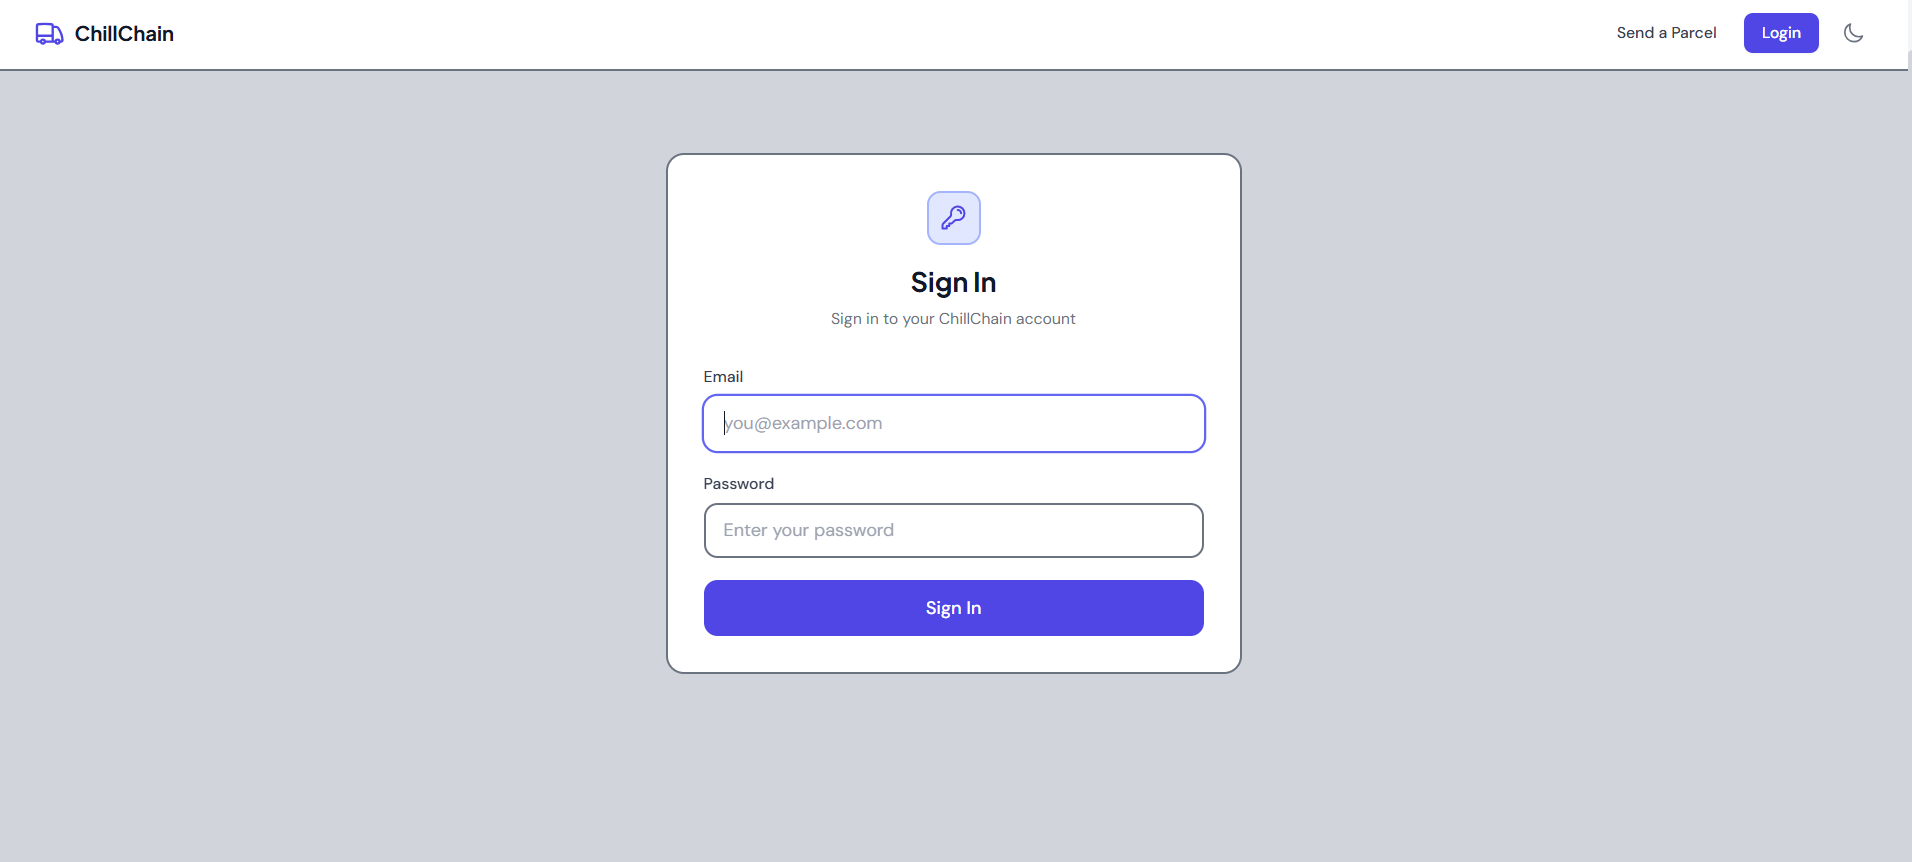
\includegraphics[width=0.95\textwidth]{img/val_login_admin.png}
\fbox{\parbox{0.9\textwidth}{\centering\vspace{3cm}\textit{Screenshot: schermata di login}\vspace{3cm}}}
\caption{Schermata di login della piattaforma. L'utente inserisce email e password; il sistema restituisce un token JWT e reindirizza alla dashboard corrispondente al ruolo.}
\label{fig:val_login}
\end{figure}

\begin{figure}[ht]
\centering
% 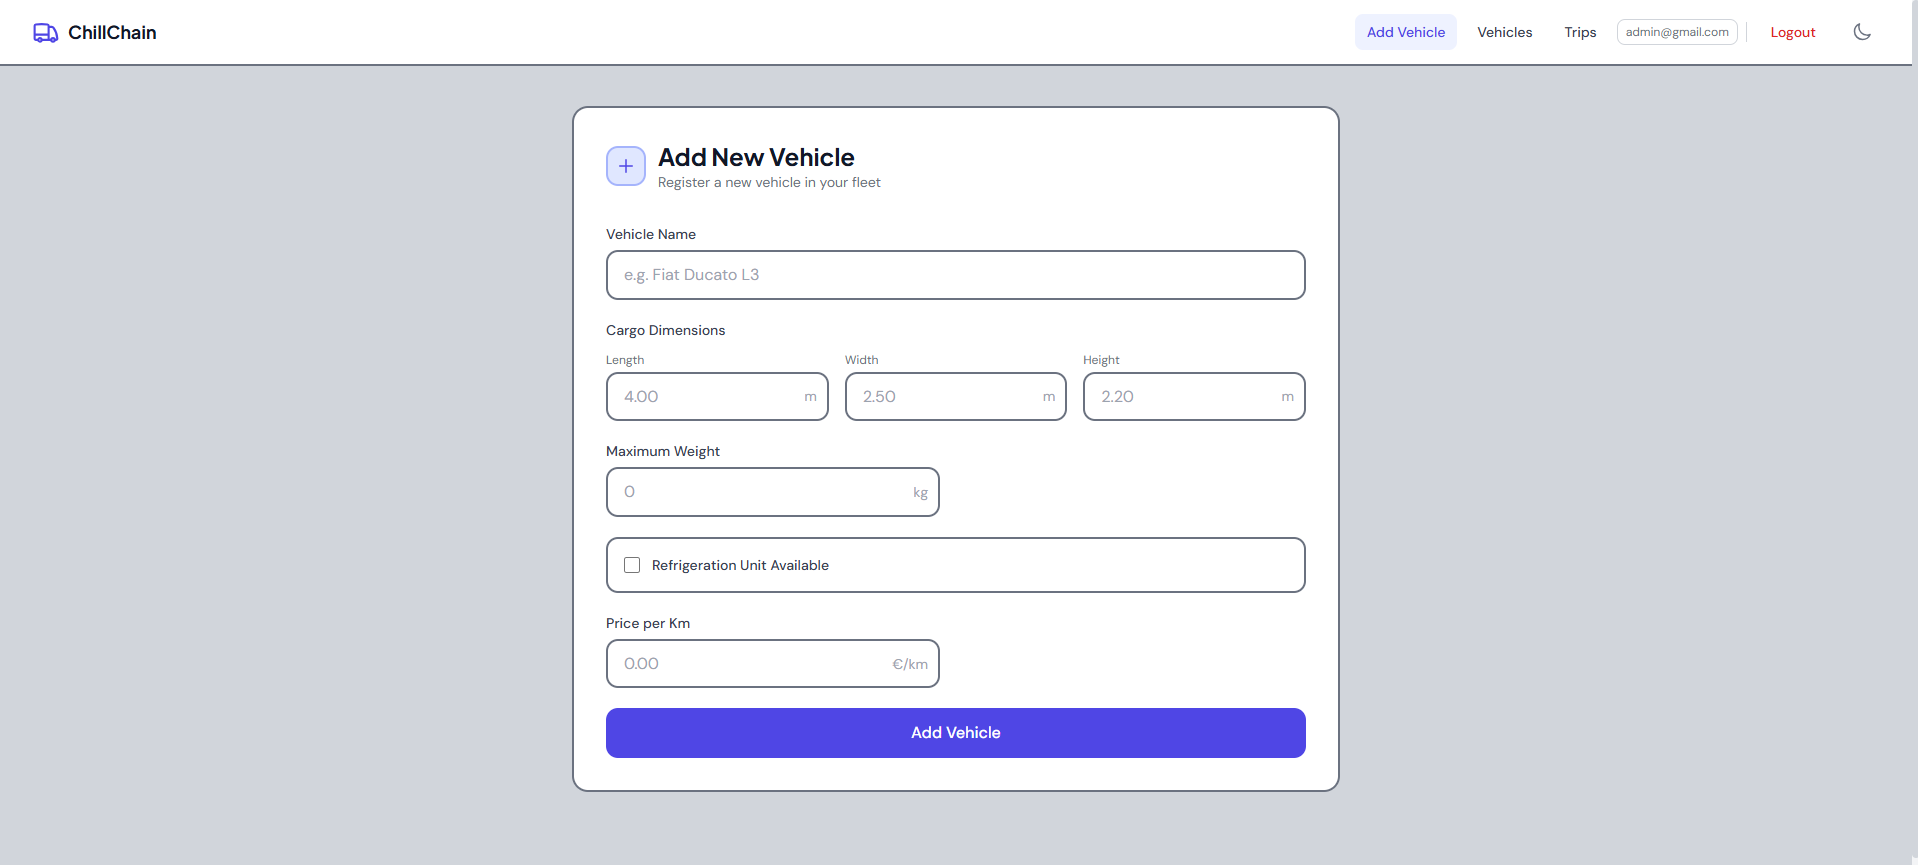
\includegraphics[width=0.95\textwidth]{img/val_add_vehicle.png}
\fbox{\parbox{0.9\textwidth}{\centering\vspace{3cm}\textit{Screenshot: form di aggiunta veicolo}\vspace{3cm}}}
\caption{Form di registrazione di un nuovo veicolo. L'amministratore specifica il nome identificativo, le dimensioni del vano di carico (larghezza, altezza, lunghezza in cm), il peso massimo trasportabile (kg), la tipologia di refrigerazione e il costo per chilometro (\euro/km).}
\label{fig:val_add_vehicle}
\end{figure}

Il primo veicolo, denominato \texttt{camion1}, è configurato con un vano di carico di 200\,$\times$\,200\,$\times$\,400~cm, peso massimo 1000~kg, refrigerazione attiva e costo di 0,50~\euro/km. Il secondo veicolo, \texttt{camion5}, ha dimensioni leggermente inferiori e un costo di 0,40~\euro/km. Entrambi i veicoli compaiono immediatamente nella lista della flotta.

\begin{figure}[ht]
\centering
% 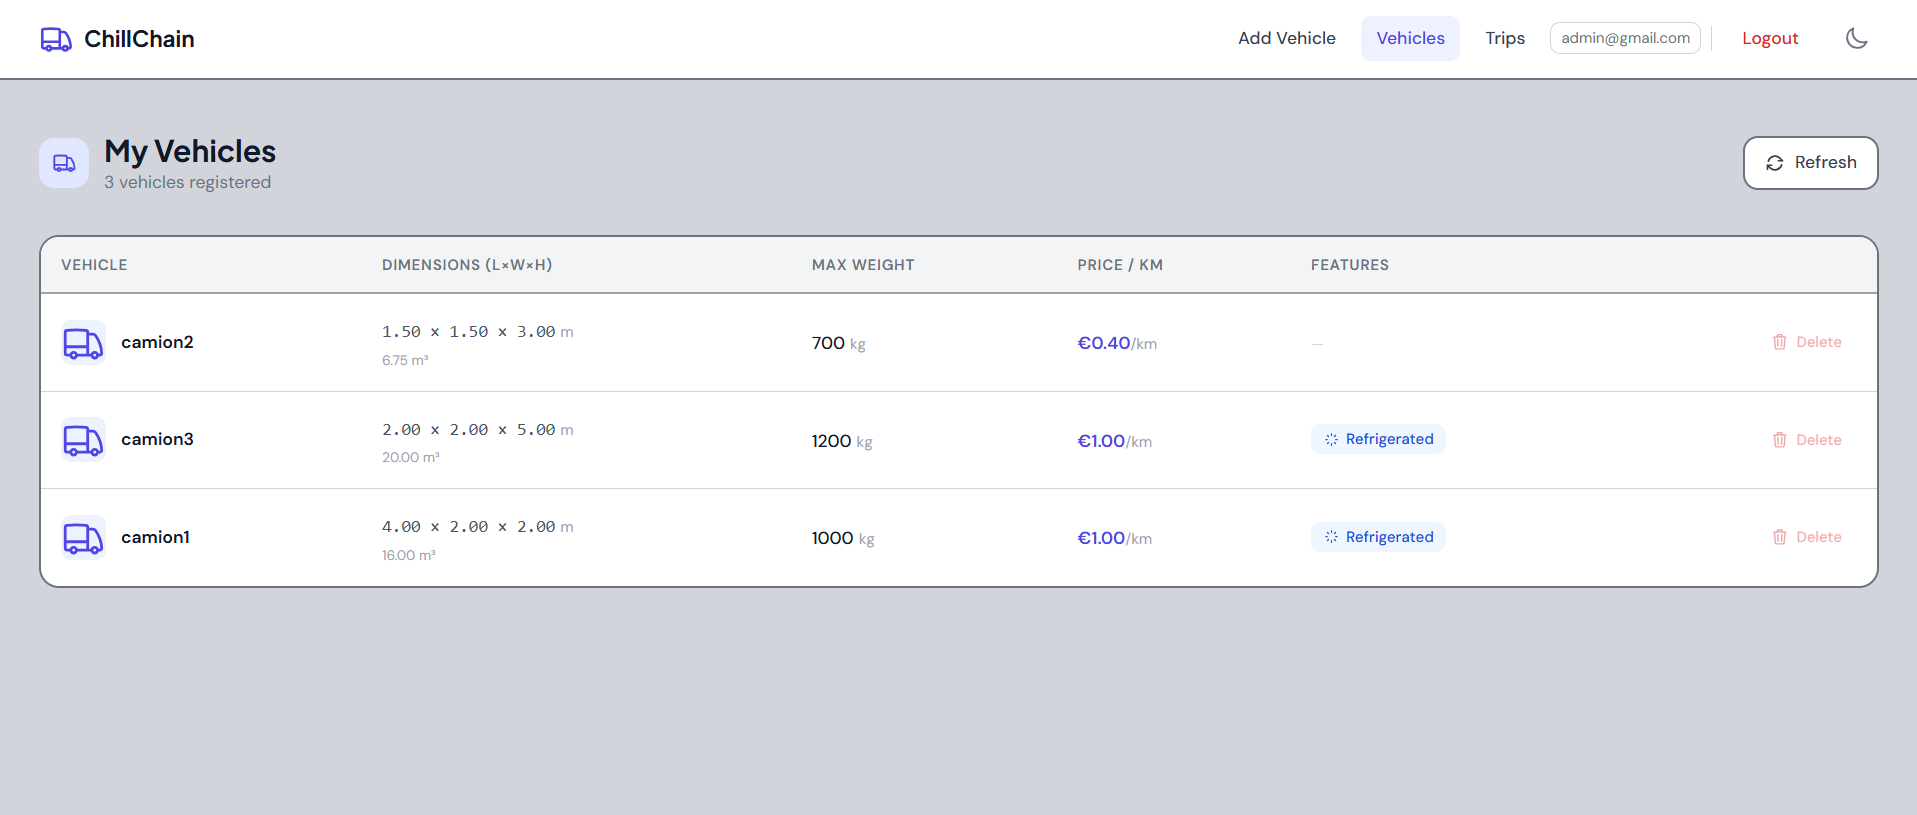
\includegraphics[width=0.95\textwidth]{img/val_vehicle_list.png}
\fbox{\parbox{0.9\textwidth}{\centering\vspace{3cm}\textit{Screenshot: lista veicoli della flotta}\vspace{3cm}}}
\caption{Lista dei veicoli registrati nella flotta. Per ciascun veicolo sono visualizzati il nome, le dimensioni, il peso massimo, lo stato di refrigerazione e il prezzo per chilometro. Le azioni disponibili includono l'eliminazione del veicolo e la visualizzazione delle tratte associate.}
\label{fig:val_vehicle_list}
\end{figure}


% ----------------------------------------------------------------------------
\subsection{Fase 2 --- Prima spedizione: creazione della tratta (Cliente A)}
\label{subsec:fase2}

Un primo cliente accede alla piattaforma e inserisce i dati della propria spedizione: partenza da Milano, arrivo a Roma, pacco di 50\,$\times$\,50\,$\times$\,50~cm con peso di 100~kg, refrigerazione necessaria e data di arrivo entro il 28 febbraio 2026.

\begin{figure}[ht]
\centering
% 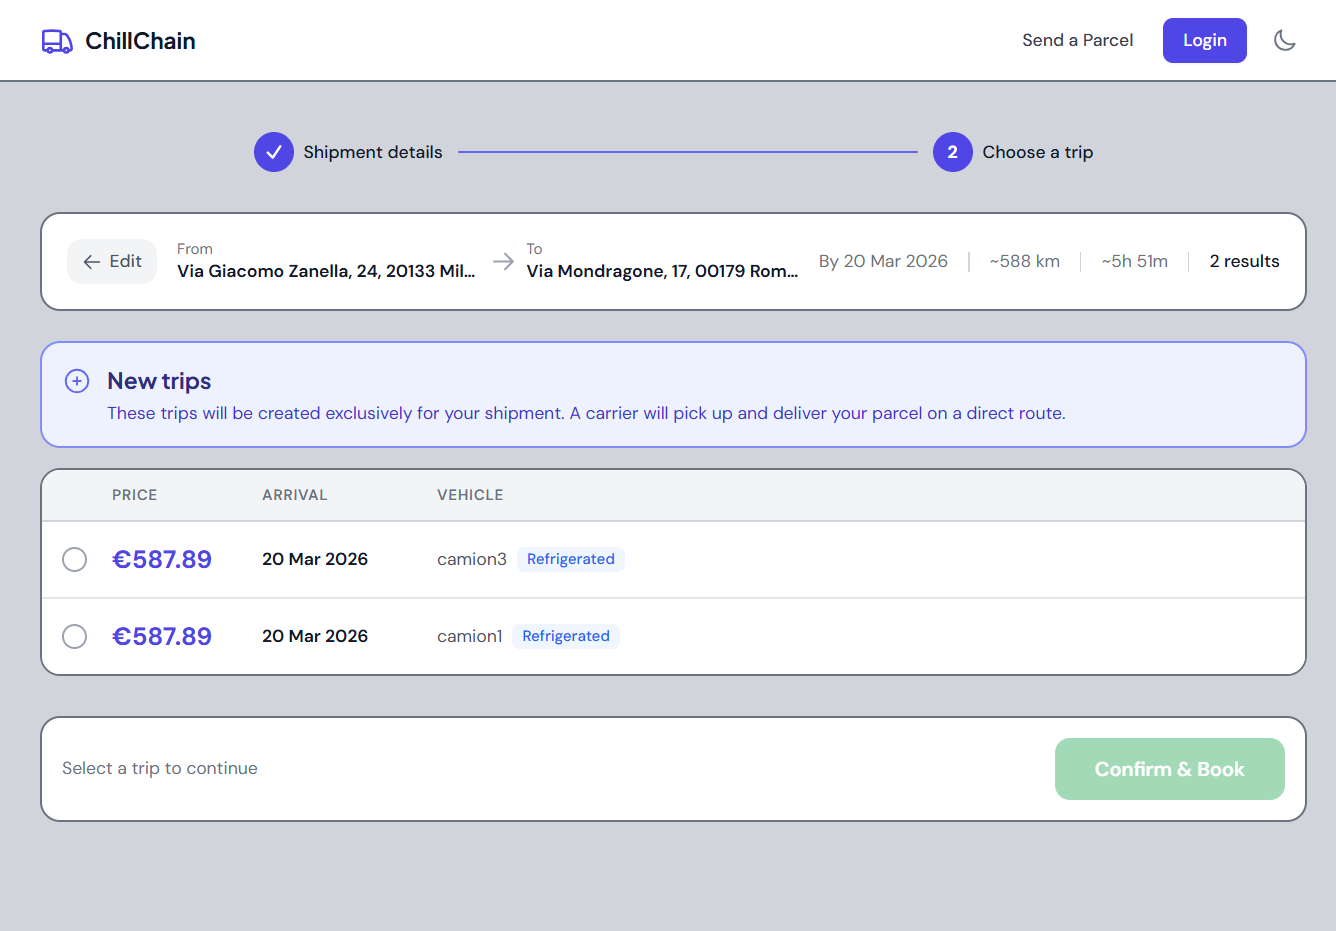
\includegraphics[width=0.95\textwidth]{img/val_send_parcel.png}
\fbox{\parbox{0.9\textwidth}{\centering\vspace{3cm}\textit{Screenshot: form di invio spedizione}\vspace{3cm}}}
\caption{Form di ricerca tratte. Il cliente inserisce gli indirizzi di partenza e arrivo, le dimensioni e il peso del pacco, la necessità di refrigerazione e la data di arrivo desiderata.}
\label{fig:val_send_parcel}
\end{figure}

Il sistema restituisce la lista delle tratte disponibili. In questo caso, poiché nessun veicolo ha ancora una tratta assegnata, vengono mostrati entrambi i veicoli come opzioni ``vuote'': \texttt{camion1} a 287,50~\euro{} e \texttt{camion5} a 230,00~\euro{} (calcolati come distanza Milano--Roma $\times$ prezzo/km del rispettivo veicolo). Per ciascuna opzione, il cliente può visualizzare il percorso su mappa prima di confermare.

\begin{figure}[ht]
\centering
% 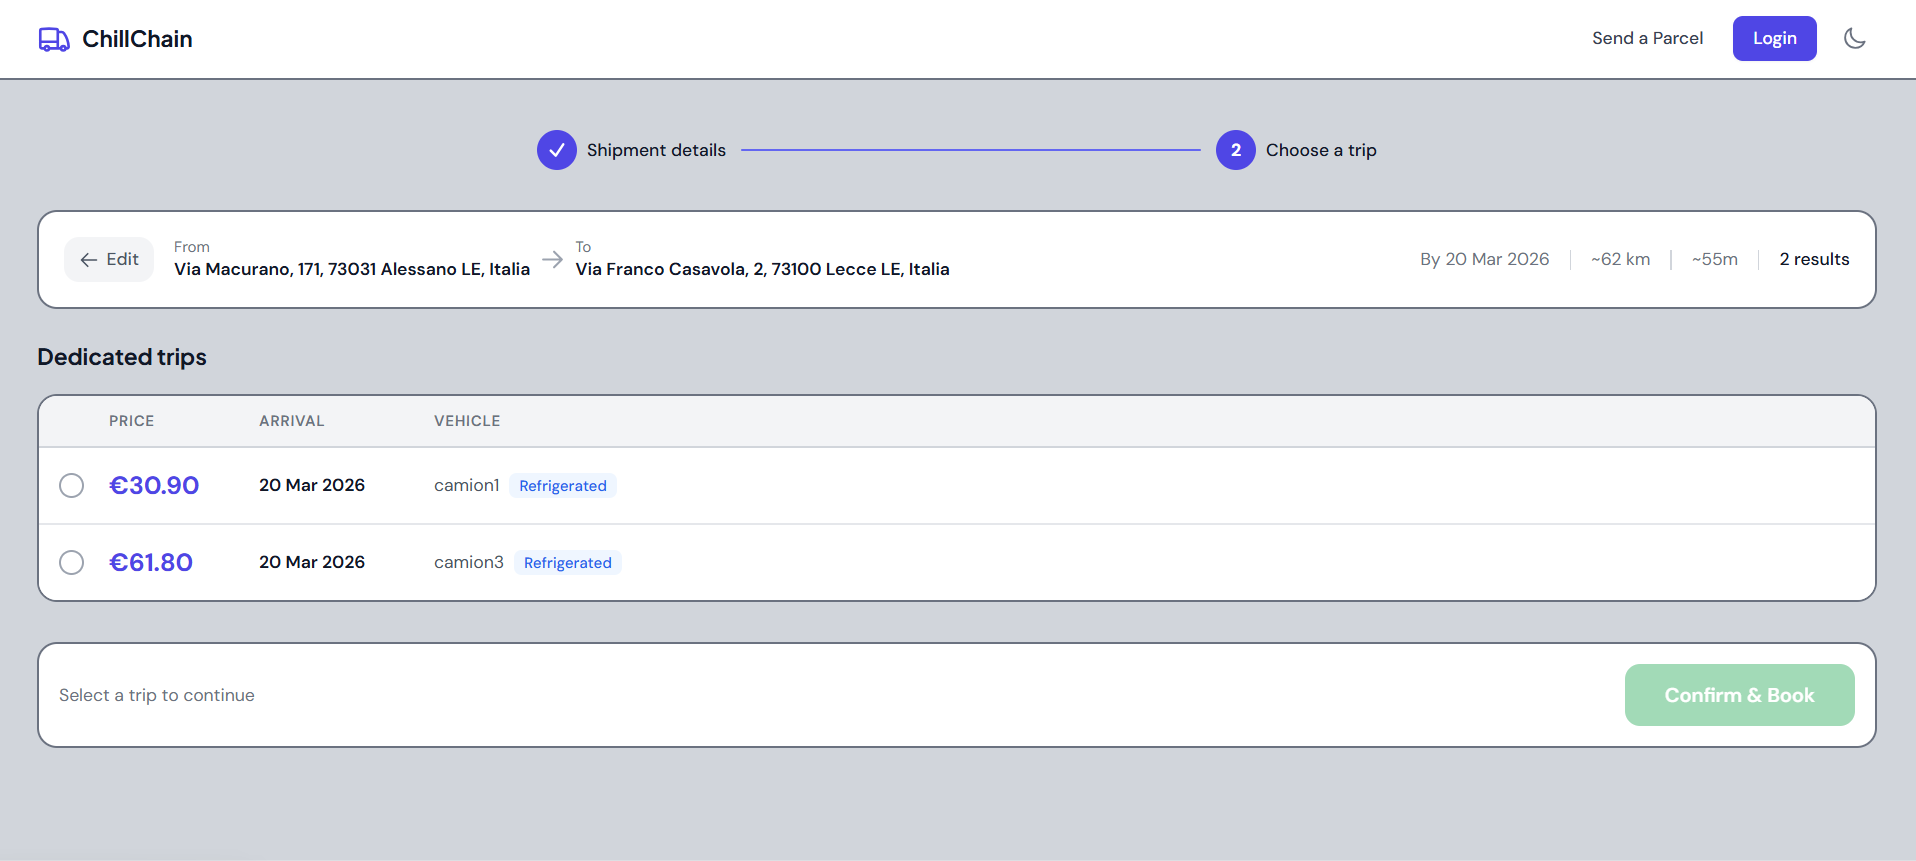
\includegraphics[width=0.95\textwidth]{img/val_trip_list_first.png}
\fbox{\parbox{0.9\textwidth}{\centering\vspace{3cm}\textit{Screenshot: lista tratte disponibili con mappa}\vspace{3cm}}}
\caption{Risultati della ricerca tratte per il Cliente A. Sono visibili due veicoli disponibili con il percorso Milano--Roma, prezzo calcolato, distanza e durata stimata. La mappa mostra la polyline del percorso selezionato.}
\label{fig:val_trip_list_first}
\end{figure}

Il Cliente A seleziona \texttt{camion1}. Il backend crea una nuova entità \texttt{Trip} con il percorso Milano--Roma, decrementa la capacità residua del veicolo e salva lo \texttt{Shipment} associato.


% ----------------------------------------------------------------------------
\subsection{Fase 3 --- Seconda spedizione: condivisione della tratta (Cliente B)}
\label{subsec:fase3}

Un secondo cliente effettua una ricerca per una spedizione da Bologna a Firenze, con un pacco più piccolo (30\,$\times$\,30\,$\times$\,30~cm, 20~kg, refrigerato, stesso periodo di arrivo).

\begin{figure}[ht]
\centering
% 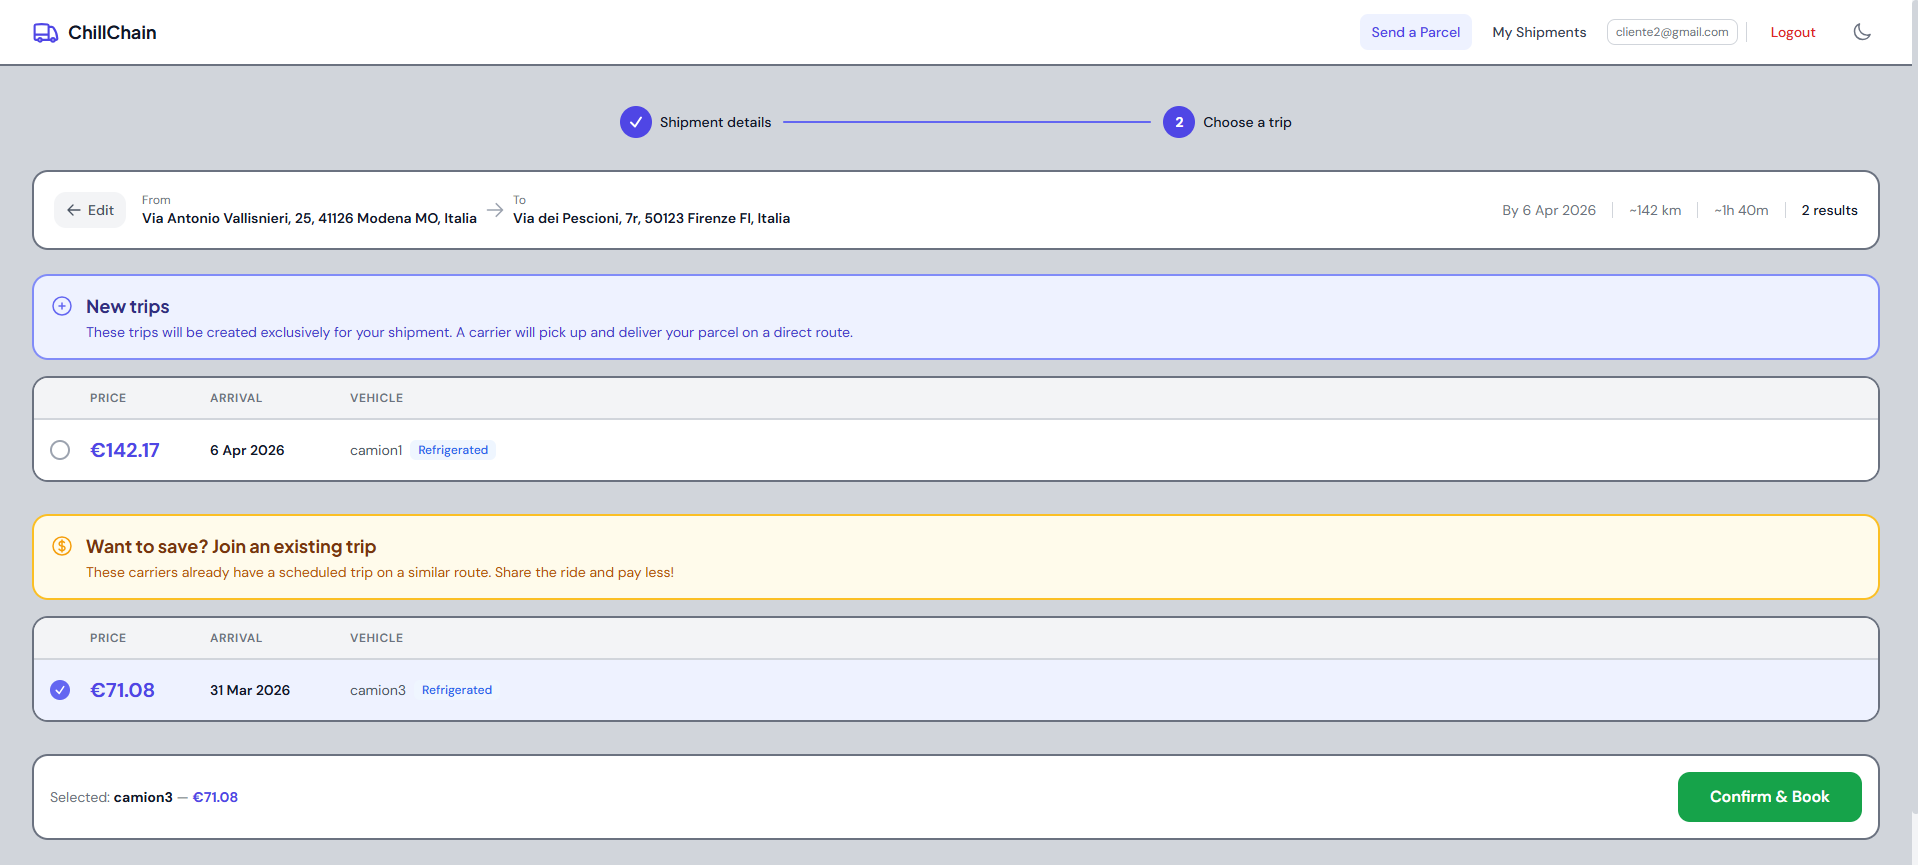
\includegraphics[width=0.95\textwidth]{img/val_trip_list_shared.png}
\fbox{\parbox{0.9\textwidth}{\centering\vspace{3cm}\textit{Screenshot: lista tratte con opzione condivisa}\vspace{3cm}}}
\caption{Risultati della ricerca tratte per il Cliente B. Oltre al veicolo \texttt{camion5} disponibile come tratta dedicata, compare \texttt{camion1} come tratta condivisa: il percorso Milano--Roma passa sufficientemente vicino a Bologna e Firenze, la deviazione rientra nei 30 minuti di tolleranza e il prezzo è scontato del 50\% grazie alla formula $2^n$ con $n=1$ spedizione già presente.}
\label{fig:val_trip_list_shared}
\end{figure}

Il sistema mostra tre opzioni: \texttt{camion5} come tratta dedicata (Bologna--Firenze a 46,00~\euro{}), \texttt{camion1} come tratta condivisa (il percorso ricalcolato Milano--Bologna--Firenze--Roma rientra nella tolleranza di 30 minuti, al prezzo scontato grazie al divisore $2^1$), e un'eventuale ulteriore opzione dedicata. Il Cliente B seleziona la tratta condivisa su \texttt{camion1}. Il backend aggiorna la polyline del trip con i nuovi waypoint (Bologna e Firenze come tappe intermedie), decrementa ulteriormente la capacità residua e salva il nuovo \texttt{Shipment}.


% ----------------------------------------------------------------------------
\subsection{Fase 4 --- Gestione della tratta e avvio simulazione (Amministratore)}
\label{subsec:fase4}

L'amministratore verifica che la tratta sia stata correttamente aggiornata, visualizzando nella sezione tratte il percorso ricalcolato con i waypoint intermedi e la lista delle spedizioni associate.

\begin{figure}[ht]
\centering
% 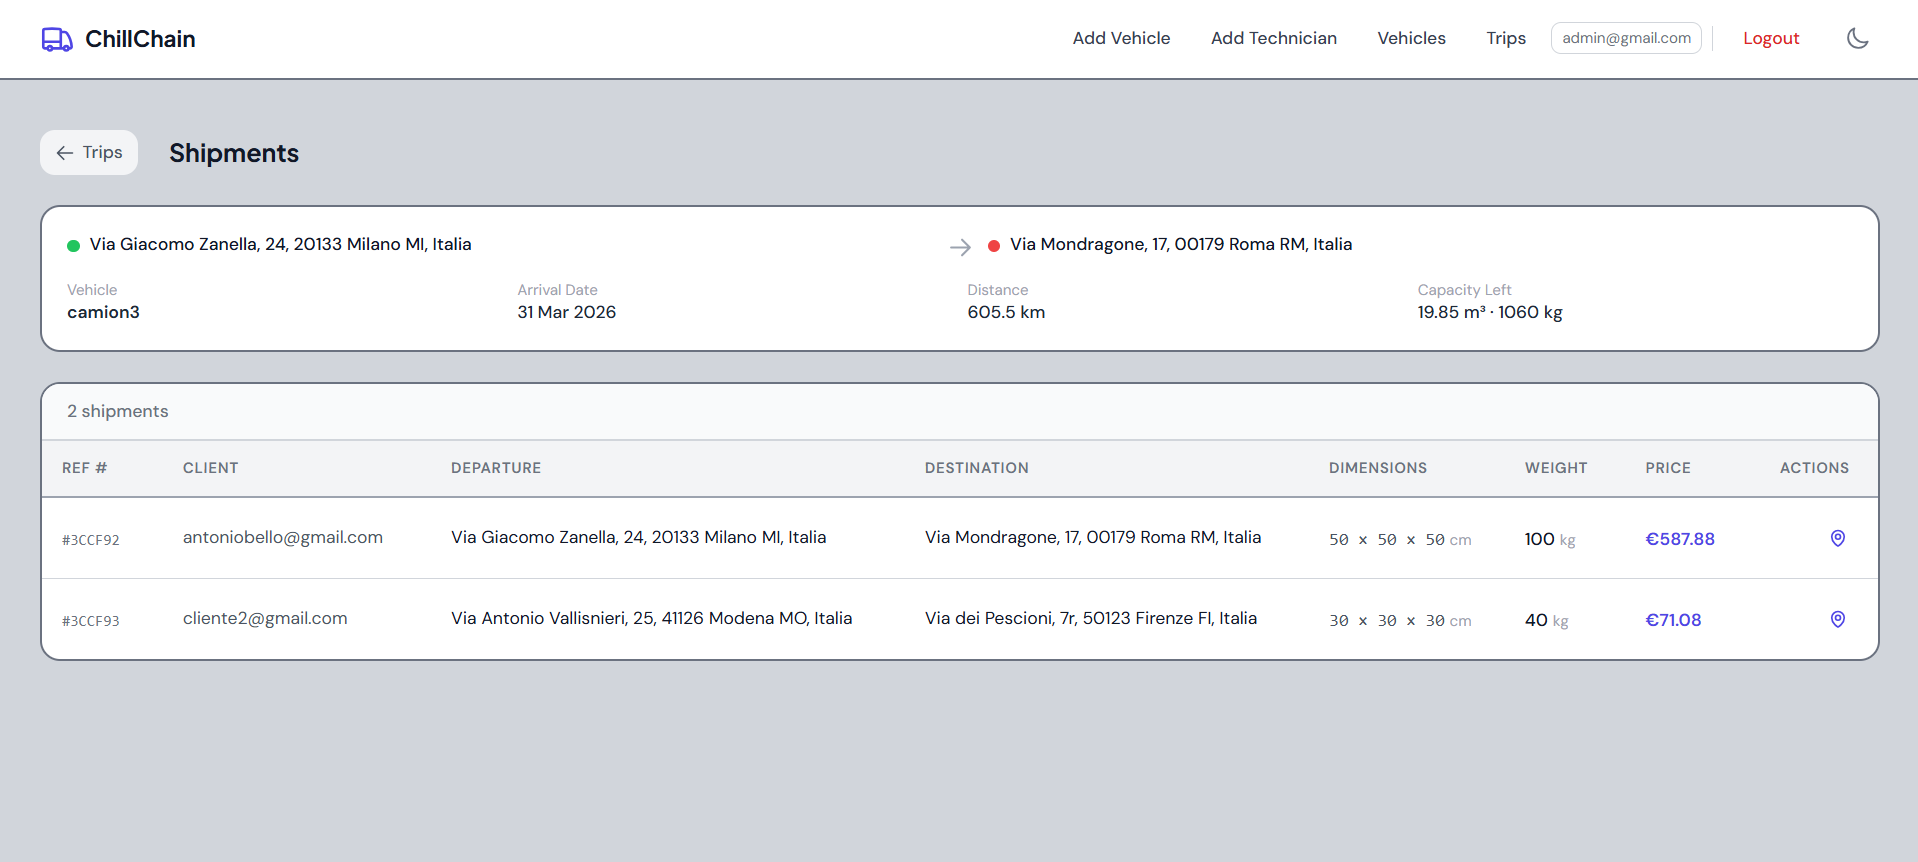
\includegraphics[width=0.95\textwidth]{img/val_trip_detail.png}
\fbox{\parbox{0.9\textwidth}{\centering\vspace{3cm}\textit{Screenshot: dettaglio tratta con spedizioni}\vspace{3cm}}}
\caption{Dettaglio della tratta assegnata a \texttt{camion1}, con il percorso aggiornato (Milano--Bologna--Firenze--Roma) e la lista delle due spedizioni associate. Sono visibili la distanza totale aggiornata, la durata e la capacità residua del veicolo.}
\label{fig:val_trip_detail}
\end{figure}

L'amministratore avvia quindi la simulazione della telemetria per \texttt{camion5}, associato al dataset contenente il guasto combinato. Il backend inoltra la richiesta al servizio di streaming, che inizia a pubblicare i dati sul topic \texttt{fridge/camion5/telemetry}.

\begin{figure}[ht]
\centering
% \includegraphics[width=0.95\textwidth]{img/val_start_simulation.png}
\fbox{\parbox{0.9\textwidth}{\centering\vspace{3cm}\textit{Screenshot: avvio simulazione telemetrica}\vspace{3cm}}}
\caption{Avvio della simulazione telemetrica per il veicolo \texttt{camion5}. Il pulsante ``Start Simulation'' attiva lo streaming dei dati dal CSV al broker MQTT. Lo stato della simulazione mostra il progresso (riga corrente/totale).}
\label{fig:val_start_simulation}
\end{figure}


% ----------------------------------------------------------------------------
\subsection{Fase 5 --- Rilevazione anomalia e notifica (Tecnico)}
\label{subsec:fase5}

Il tecnico accede alla piattaforma con le proprie credenziali e viene indirizzato alla dashboard di monitoraggio. Durante i primi 60 minuti simulati, il modello LSTM Autoencoder ricostruisce correttamente le sequenze: l'errore di ricostruzione oscilla intorno a valori di 0,005--0,008, ben al di sotto della soglia configurata.

\begin{figure}[ht]
\centering
% \includegraphics[width=0.95\textwidth]{img/val_telemetry_normal.png}
\fbox{\parbox{0.9\textwidth}{\centering\vspace{3cm}\textit{Screenshot: dashboard telemetrica in condizioni normali}\vspace{3cm}}}
\caption{Dashboard telemetrica del veicolo \texttt{camion5} durante la fase di funzionamento normale (primi 60 minuti). I grafici mostrano i parametri operativi dell'impianto frigorifero: la temperatura della cella ($T_{\text{cab\_meas}}$) oscilla intorno al setpoint, il COP è stabile e le pressioni sono nel range atteso.}
\label{fig:val_telemetry_normal}
\end{figure}

A partire dal minuto 60, il dataset inietta il guasto \texttt{UNDERCHARGE\_AND\_COND\_FOUL}: il sottocaricamento del refrigerante causa un aumento del surriscaldamento e una riduzione della capacità frigorifera, mentre il fouling del condensatore innalza la temperatura e la pressione di condensazione. Il modello inizia a produrre errori di ricostruzione superiori alla soglia. Dopo 20 campioni consecutivi anomali (il meccanismo di smoothing), il servizio di anomaly detection pubblica un messaggio di allerta sul topic \texttt{fridge/camion5/anomalies}.

Il backend riceve il messaggio, crea una notifica persistente e la rende disponibile al tecnico. L'icona delle notifiche nell'header si aggiorna con il badge numerico.

\begin{figure}[ht]
\centering
% 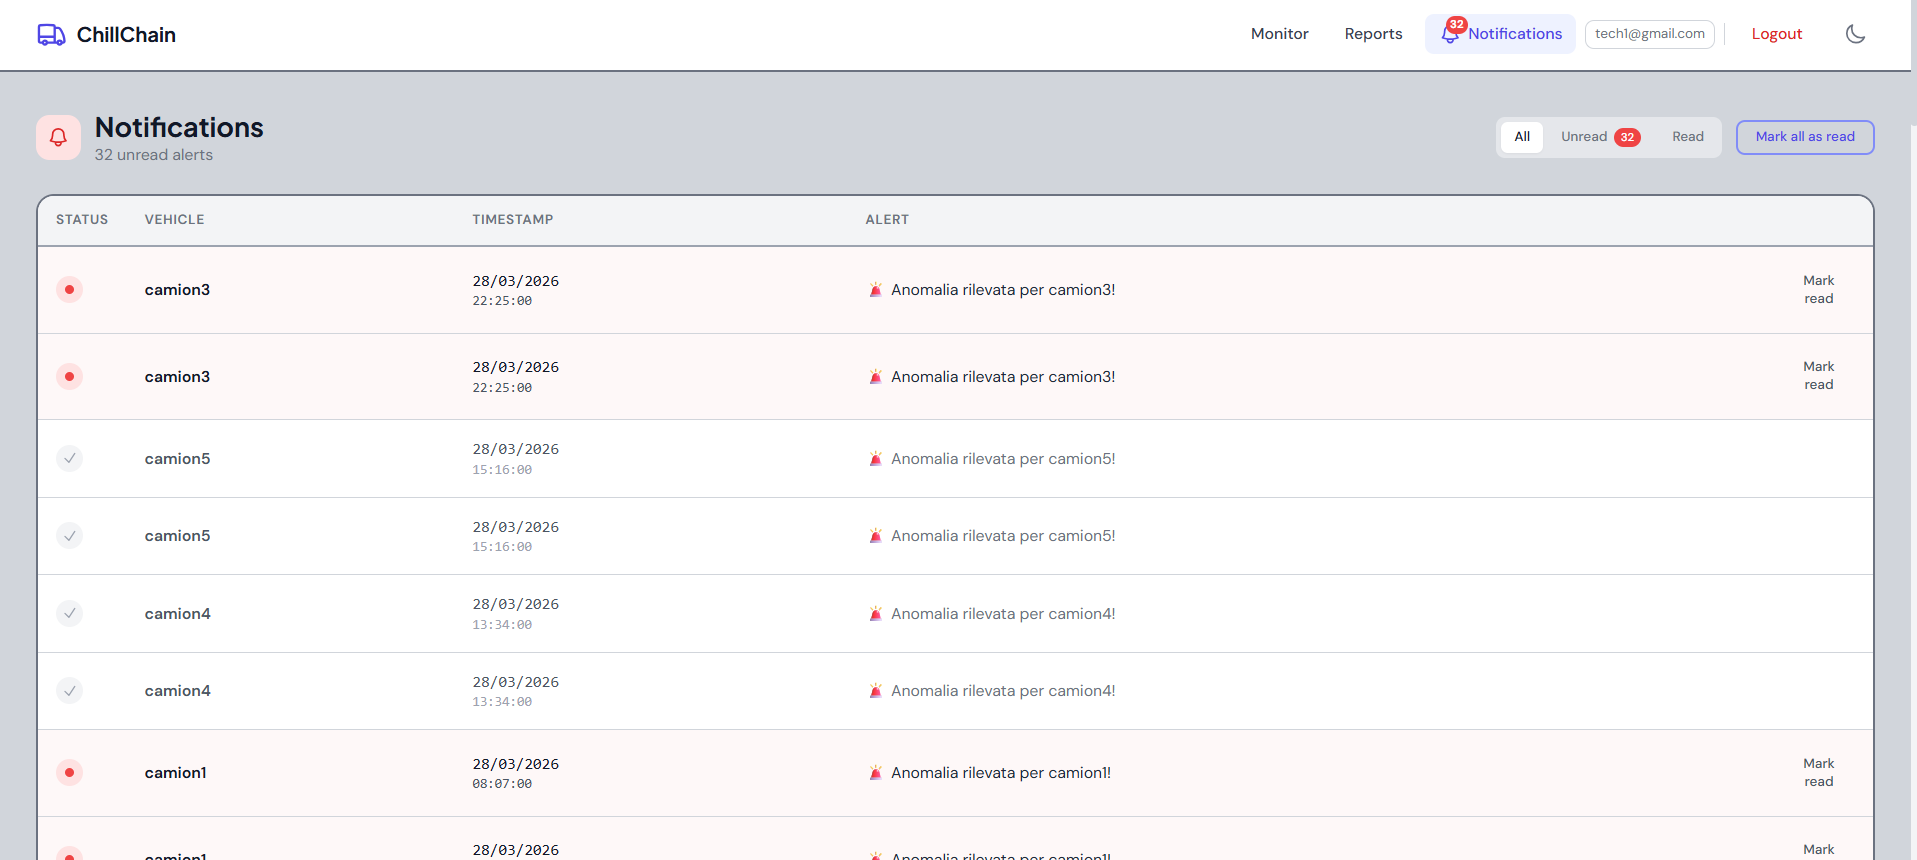
\includegraphics[width=0.95\textwidth]{img/val_notification.png}
\fbox{\parbox{0.9\textwidth}{\centering\vspace{3cm}\textit{Screenshot: notifica di anomalia ricevuta}\vspace{3cm}}}
\caption{Pannello notifiche del tecnico. La notifica indica il veicolo interessato (\texttt{camion5}), il timestamp dell'allerta, l'errore di ricostruzione e il messaggio ``Anomalia rilevata per camion5!''. Il badge nell'header mostra il conteggio delle notifiche non lette.}
\label{fig:val_notification}
\end{figure}

Il tecnico seleziona la notifica e accede alla dashboard telemetrica di \texttt{camion5}. I grafici mostrano chiaramente la transizione: intorno al campione 60, la temperatura della cella inizia a salire, il COP diminuisce, la pressione di scarico aumenta e il surriscaldamento cresce sensibilmente.

\begin{figure}[ht]
\centering
% 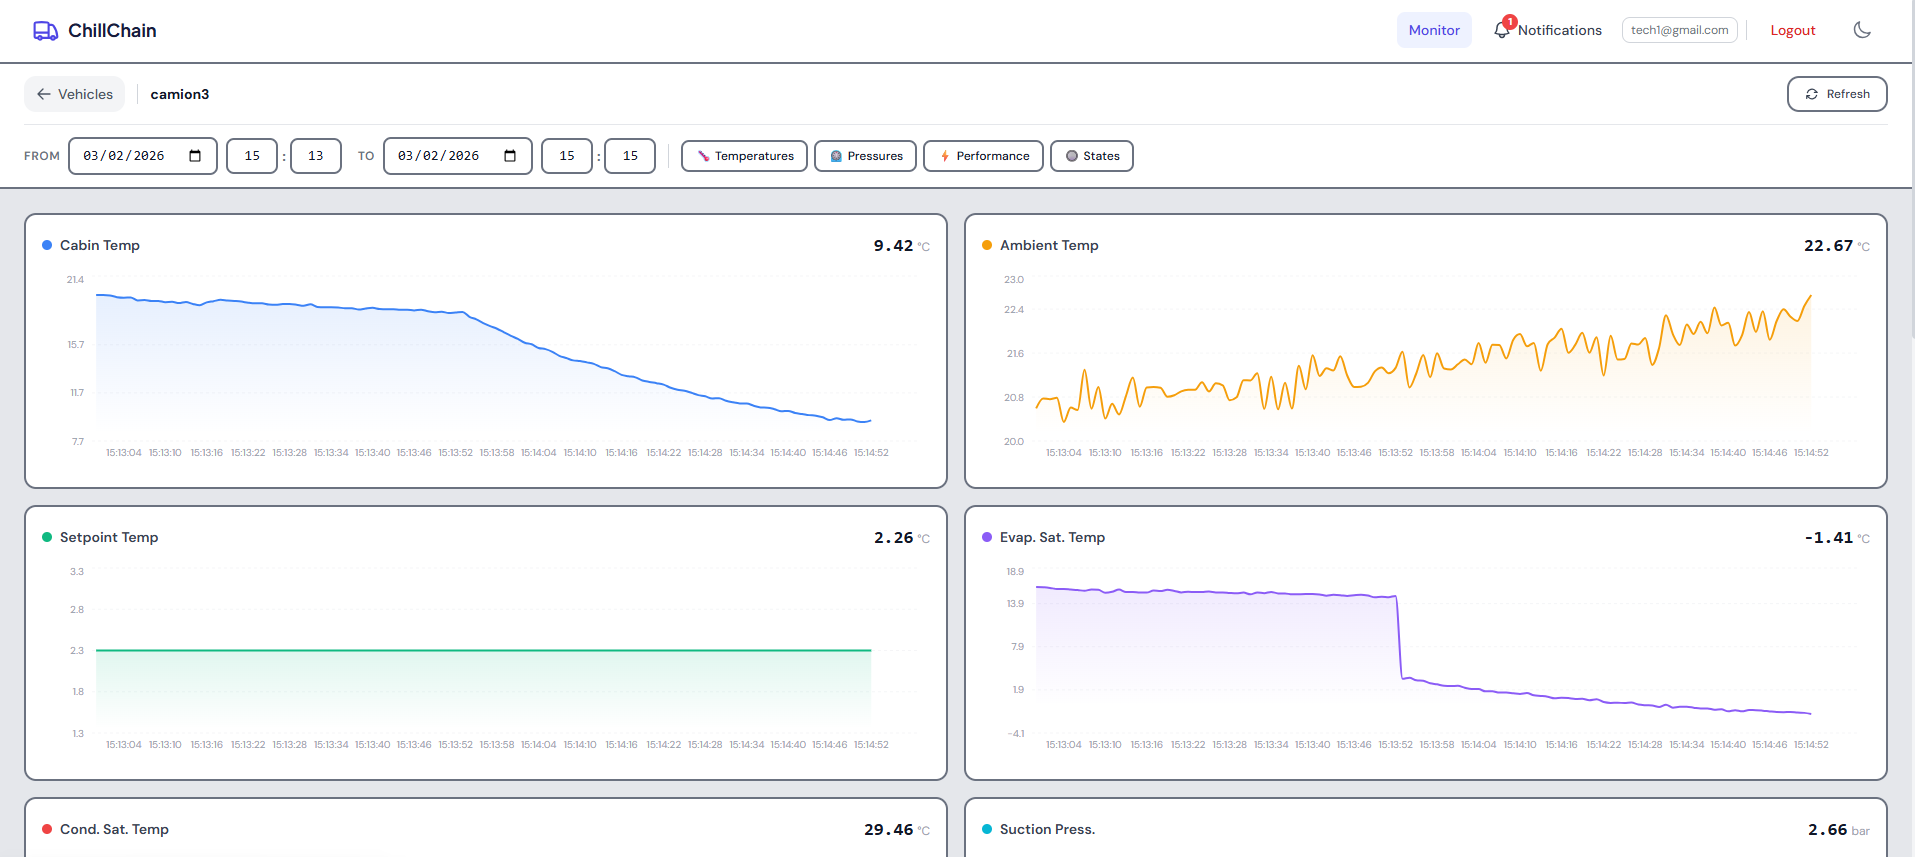
\includegraphics[width=0.95\textwidth]{img/val_telemetry_anomaly.png}
\fbox{\parbox{0.9\textwidth}{\centering\vspace{3cm}\textit{Screenshot: dashboard telemetrica con anomalia visibile}\vspace{3cm}}}
\caption{Dashboard telemetrica del veicolo \texttt{camion5} dopo l'iniezione del guasto. A partire dal campione 60, i grafici evidenziano il degrado delle prestazioni: innalzamento di $T_{\text{cab\_meas}}$ e $T_{\text{cond\_sat}}$, aumento di $P_{\text{dis\_bar}}$ e $SH_K$, riduzione del COP. La codifica cromatica passa dal verde al rosso nella zona anomala.}
\label{fig:val_telemetry_anomaly}
\end{figure}


% ============================================================================
\section{Esito della validazione}
\label{sec:esito}

Lo scenario descritto ha permesso di verificare il corretto funzionamento di tutte le funzionalità della piattaforma lungo l'intero flusso operativo.

Per quanto riguarda il marketplace, la registrazione dei veicoli, la ricerca delle tratte con filtro dimensionale e temporale, il ricalcolo del percorso con waypoint e il pricing con divisore esponenziale hanno prodotto risultati coerenti con le attese: il prezzo della tratta condivisa è risultato effettivamente dimezzato rispetto a quello della tratta dedicata, e la polyline aggiornata ha incluso correttamente le tappe intermedie di Bologna e Firenze.

Sul versante del monitoraggio, il modello LSTM Autoencoder ha ricostruito correttamente le sequenze normali (errore sotto soglia per i primi 60 minuti) e ha rilevato il degrado delle prestazioni a partire dal minuto 60. Il meccanismo di smoothing ha evitato falsi positivi durante la fase normale e ha generato la notifica circa 20 minuti dopo l'inizio del guasto, in linea con il comportamento atteso del contatore a 20 campioni consecutivi. La notifica è stata correttamente persistita su MongoDB e resa disponibile al tecnico, che ha potuto analizzare lo storico dei dati e identificare visivamente la transizione nei grafici telemetrici.

La comunicazione tra i servizi si è dimostrata affidabile: i messaggi MQTT sono stati instradati correttamente dallo streamer all'anomaly detector e da quest'ultimo al backend, senza perdita di dati osservabile. L'avvio e l'arresto della simulazione dal frontend hanno funzionato come previsto, con il messaggio di completamento che ha attivato la pulizia delle risorse del detector.

La separazione delle viste per ruolo ha operato correttamente: l'amministratore ha avuto accesso esclusivamente alla gestione della flotta e delle tratte, il cliente alla ricerca e prenotazione, il tecnico al monitoraggio e alle notifiche. Tentativi di accesso a endpoint non autorizzati hanno restituito correttamente l'errore HTTP 403.
\chapter{Conclusioni e Sviluppi Futuri}
\label{ch:conclusioni}

\section{Conclusioni}

L'obiettivo di questo lavoro era la progettazione e l'implementazione di una piattaforma IoT integrata per il trasporto refrigerato condiviso, capace di unire in un unico sistema due funzionalità tradizionalmente separate: un marketplace per il matching tra domanda e offerta di spedizioni e un sistema di monitoraggio delle condizioni del vano di refrigerazione dei veicoli con rilevazione automatica delle anomalie.


\section{Sviluppi futuri}

Nonostante i risultati ottenuti, il lavoro presenta margini di miglioramento che possono essere affrontati in sviluppi successivi.

\subsection{Ottimizzazione temporale e scheduling attivo}

L'attuale algoritmo di matching tra spedizioni e viaggi opera prevalentemente sulla dimensione spaziale, valutando la prossimità geografica tra i punti di ritiro/consegna e la polyline del percorso. La dimensione temporale, pur presente sotto forma di data di scadenza della spedizione, non viene sfruttata in modo strutturato per guidare la pianificazione dei viaggi. Un sistema più maturo potrebbe integrare le finestre di disponibilità dei trasportatori, i periodi di inattività dei veicoli e i vincoli temporali delle spedizioni in un unico modello di ottimizzazione.
\subsection{Scalabilità su piattaforme cloud}

L'attuale architettura è validata in ambiente locale tramite Docker~Compose. 
Per un utilizzo in produzione sarebbe necessario il deployment su piattaforme cloud come AWS o Azure, sfruttando servizi gestiti quali container orchestration (ECS/EKS), database managed (MongoDB~Atlas), e broker MQTT gestiti (AWS IoT~Core). Questo garantirebbe alta disponibilità, auto-scaling in funzione del carico e ridondanza geografica.

\subsection{Miglioramento della sensibilità dell'anomaly detection}

Il modello LSTM autoencoder attuale opera sulle 15~feature grezze del dataset di telemetria refrigerata. Anomalie sottili come il \emph{sensor drift}, in cui un sensore si degrada progressivamente nel tempo senza generare un errore di ricostruzione elevato su singole osservazioni, risultano difficili da rilevare con questo approccio.

Un miglioramento consiste nell'estrazione di feature derivate da fornire in input al modello.

\subsection{Indicizzazione spaziale con PostGIS}

Il calcolo della distanza punto-polyline, utilizzato per determinare la compatibilità tra un punto di ritiro/consegna e un percorso esistente, avviene attualmente con una scansione lineare $O(n)$ su tutti i segmenti della polyline decodificata. 
Questa complessità diventa un collo di bottiglia all'aumentare del numero di viaggi e della lunghezza dei percorsi.

L'adozione di PostgreSQL con l'estensione PostGIS consentirebbe di sfruttare l'indicizzazione spaziale tramite R-tree: la funzione \texttt{ST\_Distance} opera su geometrie indicizzate con complessità $O(\log n)$, riducendo drasticamente il tempo di ricerca. Inoltre, PostGIS offre nativamente operazioni come il buffer spaziale e l'intersezione tra geometrie.

\subsection{Portale cliente per il tracking delle spedizioni}

Attualmente il ruolo \texttt{CLIENT} è limitato alla fase di ricerca e prenotazione. Una volta confermata la spedizione, il cliente non dispone di strumenti per monitorarne lo stato. Un'evoluzione prevede la creazione di un'area riservata in cui il cliente possa visualizzare lo stato della spedizione in tempo reale, con stima dell'orario di arrivo calcolata sulla base della posizione corrente del veicolo e della rotta pianificata, e notifiche automatiche all'approssimarsi del ritiro o della consegna.

\subsection{Sistema di notifiche push per il tecnico}

Il sistema attuale di notifiche per anomalie è consultabile esclusivamente tramite la dashboard web: il tecnico deve accedere alla piattaforma per verificare la presenza di nuovi alert. In un contesto operativo reale, le anomalie della catena del freddo richiedono interventi tempestivi. L'integrazione di canali di notifica push, tramite email (SMTP o servizi come SendGrid) e notifiche mobile (Firebase Cloud Messaging), garantirebbe che il tecnico venga avvisato immediatamente al verificarsi di un'anomalia, indipendentemente dal fatto che stia consultando la dashboard in quel momento.


\newpage
\printbibliography

\end{document}